\pdfoutput=1
%% Author: PGL  Porta Mana
%% Created: 2019-12-15T00:46:38+0100
%% Last-Updated: 2020-02-18T14:11:20+0100
%%%%%%%%%%%%%%%%%%%%%%%%%%%%%%%%%%%%%%%%%%%%%%%%%%%%%%%%%%%%%%%%%%%%%%%%%%%%
\newif\ifarxiv
\arxivfalse
\ifarxiv\pdfmapfile{+classico.map}\fi
\newif\ifafour
\afourfalse% true = A4, false = A5
\newif\iftypodisclaim % typographical disclaim on the side
\typodisclaimtrue
\newcommand*{\memfontfamily}{zplx}
\newcommand*{\memfontpack}{newpxtext}
\documentclass[\ifafour a4paper,12pt,\else a5paper,10pt,\fi%extrafontsizes,%
onecolumn,oneside,article,%french,italian,german,swedish,latin,
british%
]{memoir}
\newcommand*{\firstdraft}{13 December 2019}%not used
\newcommand*{\firstpublished}{13 December 2019}
\newcommand*{\updated}{\ifarxiv***\else\today\fi}
\newcommand*{\propertitle}{Dimensional analysis in general relativity\\ and differential geometry%\\{\large ***}%
}% title uses LARGE; set Large for smaller
\newcommand*{\pdftitle}{\propertitle}
\newcommand*{\headtitle}{Dimensional analysis for relativity and manifolds}
\newcommand*{\pdfauthor}{P.G.L.  Porta Mana}
\newcommand*{\headauthor}{Porta Mana}
\newcommand*{\reporthead}{\iftrue\else Open Science Framework \href{https://doi.org/10.31219/osf.io/jmqnu}{\textsc{doi}:10.31219/osf.io/jmqnu}\fi}% Report number

%%%%%%%%%%%%%%%%%%%%%%%%%%%%%%%%%%%%%%%%%%%%%%%%%%%%%%%%%%%%%%%%%%%%%%%%%%%%
%%% Calls to packages (uncomment as needed)
%%%%%%%%%%%%%%%%%%%%%%%%%%%%%%%%%%%%%%%%%%%%%%%%%%%%%%%%%%%%%%%%%%%%%%%%%%%%

%\usepackage{pifont}

%\usepackage{fontawesome}

\usepackage[T1]{fontenc} 
\input{glyphtounicode} \pdfgentounicode=1

\usepackage[utf8]{inputenx}

%\usepackage{newunicodechar}
% \newunicodechar{Ĕ}{\u{E}}
% \newunicodechar{ĕ}{\u{e}}
% \newunicodechar{Ĭ}{\u{I}}
% \newunicodechar{ĭ}{\u{\i}}
% \newunicodechar{Ŏ}{\u{O}}
% \newunicodechar{ŏ}{\u{o}}
% \newunicodechar{Ŭ}{\u{U}}
% \newunicodechar{ŭ}{\u{u}}
% \newunicodechar{Ā}{\=A}
% \newunicodechar{ā}{\=a}
% \newunicodechar{Ē}{\=E}
% \newunicodechar{ē}{\=e}
% \newunicodechar{Ī}{\=I}
% \newunicodechar{ī}{\={\i}}
% \newunicodechar{Ō}{\=O}
% \newunicodechar{ō}{\=o}
% \newunicodechar{Ū}{\=U}
% \newunicodechar{ū}{\=u}
% \newunicodechar{Ȳ}{\=Y}
% \newunicodechar{ȳ}{\=y}

\newcommand*{\bmmax}{0} % reduce number of bold fonts, before font packages
\newcommand*{\hmmax}{0} % reduce number of heavy fonts, before font packages

\usepackage{textcomp}

%\usepackage[normalem]{ulem}% package for underlining
% \makeatletter
% \def\ssout{\bgroup \ULdepth=-.35ex%\UL@setULdepth
%  \markoverwith{\lower\ULdepth\hbox
%    {\kern-.03em\vbox{\hrule width.2em\kern1.2\p@\hrule}\kern-.03em}}%
%  \ULon}
% \makeatother

\usepackage{amsmath}

\usepackage{mathtools}
\addtolength{\jot}{\jot} % increase spacing in multiline formulae
\setlength{\multlinegap}{0pt}

%\usepackage{empheq}% automatically calls amsmath and mathtools
%\newcommand*{\widefbox}[1]{\fbox{\hspace{1em}#1\hspace{1em}}}

%%%% empheq above seems more versatile than these:
%\usepackage{fancybox}
%\usepackage{framed}

% \usepackage[misc]{ifsym} % for dice
% \newcommand*{\diceone}{{\scriptsize\Cube{1}}}

\usepackage{amssymb}

\usepackage{amsxtra}

\usepackage{tensor}

\usepackage[main=british,french,italian,german,swedish,latin,esperanto]{babel}\selectlanguage{british}
\newcommand*{\langfrench}{\foreignlanguage{french}}
\newcommand*{\langgerman}{\foreignlanguage{german}}
\newcommand*{\langitalian}{\foreignlanguage{italian}}
\newcommand*{\langswedish}{\foreignlanguage{swedish}}
\newcommand*{\langlatin}{\foreignlanguage{latin}}
\newcommand*{\langnohyph}{\foreignlanguage{nohyphenation}}

\usepackage[autostyle=false,autopunct=false,english=british]{csquotes}
\setquotestyle{british}

\usepackage{amsthm}
\newcommand*{\QED}{\textsc{q.e.d.}}
\renewcommand*{\qedsymbol}{\QED}
\theoremstyle{remark}
\newtheorem{note}{Note}
\newtheorem*{remark}{Note}
\newtheoremstyle{innote}{\parsep}{\parsep}{\footnotesize}{}{}{}{0pt}{}
\theoremstyle{innote}
\newtheorem*{innote}{}

\usepackage[shortlabels,inline]{enumitem}
\SetEnumitemKey{para}{itemindent=\parindent,leftmargin=0pt,listparindent=\parindent,parsep=0pt,itemsep=\topsep}
% \begin{asparaenum} = \begin{enumerate}[para]
% \begin{inparaenum} = \begin{enumerate*}
\setlist{itemsep=0pt,topsep=\parsep}
\setlist[enumerate,2]{label=\alph*.}
\setlist[enumerate]{label=\arabic*.,leftmargin=1.5\parindent}
\setlist[itemize]{leftmargin=1.5\parindent}
\setlist[description]{leftmargin=1.5\parindent}
% old alternative:
% \setlist[enumerate,2]{label=\alph*.}
% \setlist[enumerate]{leftmargin=\parindent}
% \setlist[itemize]{leftmargin=\parindent}
% \setlist[description]{leftmargin=\parindent}

\usepackage[babel,theoremfont,largesc]{newpxtext}

\usepackage[bigdelims,nosymbolsc%,smallerops % probably arXiv doesn't have it
]{newpxmath}
\linespread{1.083}%\useosf
%% smaller operators for old version of newpxmath
\makeatletter
\def\re@DeclareMathSymbol#1#2#3#4{%
    \let#1=\undefined
    \DeclareMathSymbol{#1}{#2}{#3}{#4}}
%\re@DeclareMathSymbol{\bigsqcupop}{\mathop}{largesymbols}{"46}
%\re@DeclareMathSymbol{\bigodotop}{\mathop}{largesymbols}{"4A}
\re@DeclareMathSymbol{\bigoplusop}{\mathop}{largesymbols}{"4C}
\re@DeclareMathSymbol{\bigotimesop}{\mathop}{largesymbols}{"4E}
\re@DeclareMathSymbol{\sumop}{\mathop}{largesymbols}{"50}
\re@DeclareMathSymbol{\prodop}{\mathop}{largesymbols}{"51}
\re@DeclareMathSymbol{\bigcupop}{\mathop}{largesymbols}{"53}
\re@DeclareMathSymbol{\bigcapop}{\mathop}{largesymbols}{"54}
%\re@DeclareMathSymbol{\biguplusop}{\mathop}{largesymbols}{"55}
\re@DeclareMathSymbol{\bigwedgeop}{\mathop}{largesymbols}{"56}
\re@DeclareMathSymbol{\bigveeop}{\mathop}{largesymbols}{"57}
%\re@DeclareMathSymbol{\bigcupdotop}{\mathop}{largesymbols}{"DF}
%\re@DeclareMathSymbol{\bigcapplusop}{\mathop}{largesymbolsPXA}{"00}
%\re@DeclareMathSymbol{\bigsqcupplusop}{\mathop}{largesymbolsPXA}{"02}
%\re@DeclareMathSymbol{\bigsqcapplusop}{\mathop}{largesymbolsPXA}{"04}
%\re@DeclareMathSymbol{\bigsqcapop}{\mathop}{largesymbolsPXA}{"06}
\re@DeclareMathSymbol{\bigtimesop}{\mathop}{largesymbolsPXA}{"10}
%\re@DeclareMathSymbol{\coprodop}{\mathop}{largesymbols}{"60}
%\re@DeclareMathSymbol{\varprod}{\mathop}{largesymbolsPXA}{16}
\makeatother
%%
%% With euler font cursive for Greek letters - the [1] means 100% scaling
\DeclareFontFamily{U}{egreek}{\skewchar\font'177}%
\DeclareFontShape{U}{egreek}{m}{n}{<-6>s*[1]eurm5 <6-8>s*[1]eurm7 <8->s*[1]eurm10}{}%
\DeclareFontShape{U}{egreek}{m}{it}{<->s*[1]eurmo10}{}%
\DeclareFontShape{U}{egreek}{b}{n}{<-6>s*[1]eurb5 <6-8>s*[1]eurb7 <8->s*[1]eurb10}{}%
\DeclareFontShape{U}{egreek}{b}{it}{<->s*[1]eurbo10}{}%
\DeclareSymbolFont{egreeki}{U}{egreek}{m}{it}%
\SetSymbolFont{egreeki}{bold}{U}{egreek}{b}{it}% from the amsfonts package
\DeclareSymbolFont{egreekr}{U}{egreek}{m}{n}%
\SetSymbolFont{egreekr}{bold}{U}{egreek}{b}{n}% from the amsfonts package
% Take also \sum, \prod, \coprod symbols from Euler fonts
\DeclareFontFamily{U}{egreekx}{\skewchar\font'177}
\DeclareFontShape{U}{egreekx}{m}{n}{%
       <-7.5>s*[0.9]euex7%
    <7.5-8.5>s*[0.9]euex8%
    <8.5-9.5>s*[0.9]euex9%
    <9.5->s*[0.9]euex10%
}{}
\DeclareSymbolFont{egreekx}{U}{egreekx}{m}{n}
\DeclareMathSymbol{\sumop}{\mathop}{egreekx}{"50}
\DeclareMathSymbol{\prodop}{\mathop}{egreekx}{"51}
\DeclareMathSymbol{\coprodop}{\mathop}{egreekx}{"60}
\makeatletter
\def\sum{\DOTSI\sumop\slimits@}
\def\prod{\DOTSI\prodop\slimits@}
\def\coprod{\DOTSI\coprodop\slimits@}
\makeatother
% Greek letters not usually given in LaTeX.
\DeclareMathSymbol{\varpartial}{\mathalpha}{egreeki}{"40}
\DeclareMathSymbol{\partialup}{\mathalpha}{egreekr}{"40}
\DeclareMathSymbol{\alpha}{\mathalpha}{egreeki}{"0B}
\DeclareMathSymbol{\beta}{\mathalpha}{egreeki}{"0C}
\DeclareMathSymbol{\gamma}{\mathalpha}{egreeki}{"0D}
\DeclareMathSymbol{\delta}{\mathalpha}{egreeki}{"0E}
\DeclareMathSymbol{\epsilon}{\mathalpha}{egreeki}{"0F}
\DeclareMathSymbol{\zeta}{\mathalpha}{egreeki}{"10}
\DeclareMathSymbol{\eta}{\mathalpha}{egreeki}{"11}
\DeclareMathSymbol{\theta}{\mathalpha}{egreeki}{"12}
\DeclareMathSymbol{\iota}{\mathalpha}{egreeki}{"13}
\DeclareMathSymbol{\kappa}{\mathalpha}{egreeki}{"14}
\DeclareMathSymbol{\lambda}{\mathalpha}{egreeki}{"15}
\DeclareMathSymbol{\mu}{\mathalpha}{egreeki}{"16}
\DeclareMathSymbol{\nu}{\mathalpha}{egreeki}{"17}
\DeclareMathSymbol{\xi}{\mathalpha}{egreeki}{"18}
\DeclareMathSymbol{\omicron}{\mathalpha}{egreeki}{"6F}
\DeclareMathSymbol{\pi}{\mathalpha}{egreeki}{"19}
\DeclareMathSymbol{\rho}{\mathalpha}{egreeki}{"1A}
\DeclareMathSymbol{\sigma}{\mathalpha}{egreeki}{"1B}
 \DeclareMathSymbol{\tau}{\mathalpha}{egreeki}{"1C}
\DeclareMathSymbol{\upsilon}{\mathalpha}{egreeki}{"1D}
\DeclareMathSymbol{\phi}{\mathalpha}{egreeki}{"1E}
\DeclareMathSymbol{\chi}{\mathalpha}{egreeki}{"1F}
\DeclareMathSymbol{\psi}{\mathalpha}{egreeki}{"20}
\DeclareMathSymbol{\omega}{\mathalpha}{egreeki}{"21}
\DeclareMathSymbol{\varepsilon}{\mathalpha}{egreeki}{"22}
\DeclareMathSymbol{\vartheta}{\mathalpha}{egreeki}{"23}
\DeclareMathSymbol{\varpi}{\mathalpha}{egreeki}{"24}
\let\varrho\rho 
\let\varsigma\sigma
 \let\varkappa\kappa
\DeclareMathSymbol{\varphi}{\mathalpha}{egreeki}{"27}
%
\DeclareMathSymbol{\varAlpha}{\mathalpha}{egreeki}{"41}
\DeclareMathSymbol{\varBeta}{\mathalpha}{egreeki}{"42}
\DeclareMathSymbol{\varGamma}{\mathalpha}{egreeki}{"00}
\DeclareMathSymbol{\varDelta}{\mathalpha}{egreeki}{"01}
\DeclareMathSymbol{\varEpsilon}{\mathalpha}{egreeki}{"45}
\DeclareMathSymbol{\varZeta}{\mathalpha}{egreeki}{"5A}
\DeclareMathSymbol{\varEta}{\mathalpha}{egreeki}{"48}
\DeclareMathSymbol{\varTheta}{\mathalpha}{egreeki}{"02}
 \DeclareMathSymbol{\varIota}{\mathalpha}{egreeki}{"49}
\DeclareMathSymbol{\varKappa}{\mathalpha}{egreeki}{"4B}
\DeclareMathSymbol{\varLambda}{\mathalpha}{egreeki}{"03}
\DeclareMathSymbol{\varMu}{\mathalpha}{egreeki}{"4D}
\DeclareMathSymbol{\varNu}{\mathalpha}{egreeki}{"4E}
\DeclareMathSymbol{\varXi}{\mathalpha}{egreeki}{"04}
\DeclareMathSymbol{\varOmicron}{\mathalpha}{egreeki}{"4F}
\DeclareMathSymbol{\varPi}{\mathalpha}{egreeki}{"05}
\DeclareMathSymbol{\varRho}{\mathalpha}{egreeki}{"50}
\DeclareMathSymbol{\varSigma}{\mathalpha}{egreeki}{"06}
\DeclareMathSymbol{\varTau}{\mathalpha}{egreeki}{"54}
\DeclareMathSymbol{\varUpsilon}{\mathalpha}{egreeki}{"07}
\DeclareMathSymbol{\varPhi}{\mathalpha}{egreeki}{"08}
\DeclareMathSymbol{\varChi}{\mathalpha}{egreeki}{"58}
\DeclareMathSymbol{\varPsi}{\mathalpha}{egreeki}{"09}
\DeclareMathSymbol{\varOmega}{\mathalpha}{egreeki}{"0A} 
%
\DeclareMathSymbol{\Alpha}{\mathalpha}{egreekr}{"41}
\DeclareMathSymbol{\Beta}{\mathalpha}{egreekr}{"42}
\DeclareMathSymbol{\Gamma}{\mathalpha}{egreekr}{"00}
\DeclareMathSymbol{\Delta}{\mathalpha}{egreekr}{"01}
\DeclareMathSymbol{\Epsilon}{\mathalpha}{egreekr}{"45}
\DeclareMathSymbol{\Zeta}{\mathalpha}{egreekr}{"5A}
\DeclareMathSymbol{\Eta}{\mathalpha}{egreekr}{"48}
\DeclareMathSymbol{\Theta}{\mathalpha}{egreekr}{"02}
\DeclareMathSymbol{\Iota}{\mathalpha}{egreekr}{"49}
\DeclareMathSymbol{\Kappa}{\mathalpha}{egreekr}{"4B}
\DeclareMathSymbol{\Lambda}{\mathalpha}{egreekr}{"03}
\DeclareMathSymbol{\Mu}{\mathalpha}{egreekr}{"4D}
\DeclareMathSymbol{\Nu}{\mathalpha}{egreekr}{"4E}
\DeclareMathSymbol{\Xi}{\mathalpha}{egreekr}{"04}
\DeclareMathSymbol{\Omicron}{\mathalpha}{egreekr}{"4F}
\DeclareMathSymbol{\Pi}{\mathalpha}{egreekr}{"05}
\DeclareMathSymbol{\Rho}{\mathalpha}{egreekr}{"50}
\DeclareMathSymbol{\Sigma}{\mathalpha}{egreekr}{"06}
\DeclareMathSymbol{\Tau}{\mathalpha}{egreekr}{"54}
\DeclareMathSymbol{\Upsilon}{\mathalpha}{egreekr}{"07}
\DeclareMathSymbol{\Phi}{\mathalpha}{egreekr}{"08}
\DeclareMathSymbol{\Chi}{\mathalpha}{egreekr}{"58}
\DeclareMathSymbol{\Psi}{\mathalpha}{egreekr}{"09}
\DeclareMathSymbol{\Omega}{\mathalpha}{egreekr}{"0A}
%
\DeclareMathSymbol{\alphaup}{\mathalpha}{egreekr}{"0B}
\DeclareMathSymbol{\betaup}{\mathalpha}{egreekr}{"0C}
\DeclareMathSymbol{\gammaup}{\mathalpha}{egreekr}{"0D}
 \DeclareMathSymbol{\deltaup}{\mathalpha}{egreekr}{"0E}
\DeclareMathSymbol{\epsilonup}{\mathalpha}{egreekr}{"0F}
\DeclareMathSymbol{\zetaup}{\mathalpha}{egreekr}{"10}
\DeclareMathSymbol{\etaup}{\mathalpha}{egreekr}{"11}
\DeclareMathSymbol{\thetaup}{\mathalpha}{egreekr}{"12}
\DeclareMathSymbol{\iotaup}{\mathalpha}{egreekr}{"13}
\DeclareMathSymbol{\kappaup}{\mathalpha}{egreekr}{"14}
\DeclareMathSymbol{\lambdaup}{\mathalpha}{egreekr}{"15}
\DeclareMathSymbol{\muup}{\mathalpha}{egreekr}{"16}
\DeclareMathSymbol{\nuup}{\mathalpha}{egreekr}{"17}
\DeclareMathSymbol{\xiup}{\mathalpha}{egreekr}{"18}
\DeclareMathSymbol{\omicronup}{\mathalpha}{egreekr}{"6F}
  \DeclareMathSymbol{\piup}{\mathalpha}{egreekr}{"19}
\DeclareMathSymbol{\rhoup}{\mathalpha}{egreekr}{"1A}
\DeclareMathSymbol{\sigmaup}{\mathalpha}{egreekr}{"1B}
\DeclareMathSymbol{\tauup}{\mathalpha}{egreekr}{"1C}
\DeclareMathSymbol{\upsilonup}{\mathalpha}{egreekr}{"1D}
\DeclareMathSymbol{\phiup}{\mathalpha}{egreekr}{"1E}
\DeclareMathSymbol{\chiup}{\mathalpha}{egreekr}{"1F}
\DeclareMathSymbol{\psiup}{\mathalpha}{egreekr}{"20}
\DeclareMathSymbol{\omegaup}{\mathalpha}{egreekr}{"21}
\DeclareMathSymbol{\varepsilonup}{\mathalpha}{egreekr}{"22}
\DeclareMathSymbol{\varthetaup}{\mathalpha}{egreekr}{"23}
\DeclareMathSymbol{\varpiup}{\mathalpha}{egreekr}{"24}
\let\varrhoup\rhoup 
\let\varsigmaup\sigmaup
\let\varkappaup\kappaup
\DeclareMathSymbol{\varphiup}{\mathalpha}{egreekr}{"27}
% Greek letters not usually given in LaTeX.

%\usepackage%[scaled=0.9]%
%{classico}%  Optima as sans-serif font
\renewcommand\sfdefault{uop}
\DeclareMathAlphabet{\mathsf}  {T1}{\sfdefault}{m}{sl}
\SetMathAlphabet{\mathsf}{bold}{T1}{\sfdefault}{b}{sl}
\newcommand*{\mathte}[1]{\textbf{\textit{\textsf{#1}}}}
% Upright sans-serif math alphabet
% \DeclareMathAlphabet{\mathsu}  {T1}{\sfdefault}{m}{n}
% \SetMathAlphabet{\mathsu}{bold}{T1}{\sfdefault}{b}{n}

% DejaVu Mono as typewriter text
\usepackage[scaled=0.84]{DejaVuSansMono}

\usepackage{mathdots}

\usepackage[usenames]{xcolor}
% Tol (2012) colour-blind-, print-, screen-friendly colours, alternative scheme; Munsell terminology
\definecolor{mypurpleblue}{RGB}{68,119,170}
\definecolor{myblue}{RGB}{102,204,238}
\definecolor{mygreen}{RGB}{34,136,51}
\definecolor{myyellow}{RGB}{204,187,68}
\definecolor{myred}{RGB}{238,102,119}
\definecolor{myredpurple}{RGB}{170,51,119}
\definecolor{mygrey}{RGB}{187,187,187}
% Tol (2012) colour-blind-, print-, screen-friendly colours; Munsell terminology
% \definecolor{lbpurple}{RGB}{51,34,136}
% \definecolor{lblue}{RGB}{136,204,238}
% \definecolor{lbgreen}{RGB}{68,170,153}
% \definecolor{lgreen}{RGB}{17,119,51}
% \definecolor{lgyellow}{RGB}{153,153,51}
% \definecolor{lyellow}{RGB}{221,204,119}
% \definecolor{lred}{RGB}{204,102,119}
% \definecolor{lpred}{RGB}{136,34,85}
% \definecolor{lrpurple}{RGB}{170,68,153}
\definecolor{lgrey}{RGB}{221,221,221}
%\newcommand*\mycolourbox[1]{%
%\colorbox{mygrey}{\hspace{1em}#1\hspace{1em}}}
\colorlet{shadecolor}{lgrey}

\usepackage{bm}

\usepackage{microtype}

\usepackage[backend=biber,mcite,%subentry,
citestyle=authoryear-comp,bibstyle=pglpm-authoryear,autopunct=false,sorting=ny,sortcites=false,natbib=false,maxcitenames=2,maxbibnames=8,minbibnames=8,giveninits=true,uniquename=false,uniquelist=false,maxalphanames=1,block=space,hyperref=true,defernumbers=false,useprefix=true,sortupper=false,language=british,parentracker=false]{biblatex}
\DeclareSortingScheme{ny}{\sort{\field{sortname}\field{author}\field{editor}}\sort{\field{year}}}
\iffalse\makeatletter%%% replace parenthesis with brackets
\newrobustcmd*{\parentexttrack}[1]{%
  \begingroup
  \blx@blxinit
  \blx@setsfcodes
  \blx@bibopenparen#1\blx@bibcloseparen
  \endgroup}
\AtEveryCite{%
  \let\parentext=\parentexttrack%
  \let\bibopenparen=\bibopenbracket%
  \let\bibcloseparen=\bibclosebracket}
\makeatother\fi
\DefineBibliographyExtras{british}{\def\finalandcomma{\addcomma}}
\renewcommand*{\finalnamedelim}{\addspace\amp\space}
\setcounter{biburlnumpenalty}{1}
\setcounter{biburlucpenalty}{0}
\setcounter{biburllcpenalty}{1}
\DeclareDelimFormat{multicitedelim}{\addsemicolon\addspace\space}
\DeclareDelimFormat{compcitedelim}{\addsemicolon\addspace\space}
\DeclareDelimFormat{postnotedelim}{\addspace}
\ifarxiv\else\addbibresource{portamanabib.bib}\fi
\renewcommand{\bibfont}{\footnotesize}
%\appto{\citesetup}{\footnotesize}% smaller font for citations
\defbibheading{bibliography}[\bibname]{\section*{#1}\addcontentsline{toc}{section}{#1}%\markboth{#1}{#1}
}
\newcommand*{\citep}{\footcites}
\newcommand*{\citey}{\parencites*}%{\footcites}%
%\renewcommand*{\cite}{\parencite}
%\renewcommand*{\cites}{\parencites}
\providecommand{\href}[2]{#2}
\providecommand{\eprint}[2]{\texttt{\href{#1}{#2}}}
\newcommand*{\amp}{\&}
% \newcommand*{\citein}[2][]{\textnormal{\textcite[#1]{#2}}%\addtocategory{extras}{#2}
% }
\newcommand*{\citein}[2][]{\textnormal{\textcite[#1]{#2}}%\addtocategory{extras}{#2}
}
\newcommand*{\citebi}[2][]{\textcite[#1]{#2}%\addtocategory{extras}{#2}
}
\newcommand*{\subtitleproc}[1]{}
\newcommand*{\chapb}{ch.}
%
% \def\arxivp{}
% \def\mparcp{}
% \def\philscip{}
% \def\biorxivp{}
% \newcommand*{\arxivsi}{\texttt{arXiv} eprints available at \url{http://arxiv.org/}.\\}
% \newcommand*{\mparcsi}{\texttt{mp\_arc} eprints available at \url{http://www.ma.utexas.edu/mp_arc/}.\\}
% \newcommand*{\philscisi}{\texttt{philsci} eprints available at \url{http://philsci-archive.pitt.edu/}.\\}
% \newcommand*{\biorxivsi}{\texttt{bioRxiv} eprints available at \url{http://biorxiv.org/}.\\}
\newcommand*{\arxiveprint}[1]{%\global\def\arxivp{\arxivsi}%\citeauthor{0arxivcite}\addtocategory{ifarchcit}{0arxivcite}%eprint
\texttt{arXiv:\urlalt{https://arxiv.org/abs/#1}{#1}}%
%\texttt{\href{http://arxiv.org/abs/#1}{\protect\url{arXiv:#1}}}%
%\renewcommand{\arxivnote}{\texttt{arXiv} eprints available at \url{http://arxiv.org/}.}
}
\newcommand*{\mparceprint}[1]{%\global\def\mparcp{\mparcsi}%\citeauthor{0mparccite}\addtocategory{ifarchcit}{0mparccite}%eprint
\texttt{mp\_arc:\urlalt{http://www.ma.utexas.edu/mp_arc-bin/mpa?yn=#1}{#1}}%
%\texttt{\href{http://www.ma.utexas.edu/mp_arc-bin/mpa?yn=#1}{\protect\url{mp_arc:#1}}}%
%\providecommand{\mparcnote}{\texttt{mp_arc} eprints available at \url{http://www.ma.utexas.edu/mp_arc/}.}
}
\newcommand*{\haleprint}[1]{%\global\def\arxivp{\arxivsi}%\citeauthor{0arxivcite}\addtocategory{ifarchcit}{0arxivcite}%eprint
\texttt{HAL:\urlalt{https://hal.archives-ouvertes.fr/#1}{#1}}%
%\texttt{\href{http://arxiv.org/abs/#1}{\protect\url{arXiv:#1}}}%
%\renewcommand{\arxivnote}{\texttt{arXiv} eprints available at \url{http://arxiv.org/}.}
}
\newcommand*{\philscieprint}[1]{%\global\def\philscip{\philscisi}%\citeauthor{0philscicite}\addtocategory{ifarchcit}{0philscicite}%eprint
\texttt{PhilSci:\urlalt{http://philsci-archive.pitt.edu/archive/#1}{#1}}%
%\texttt{\href{http://philsci-archive.pitt.edu/archive/#1}{\protect\url{PhilSci:#1}}}%
%\providecommand{\mparcnote}{\texttt{philsci} eprints available at \url{http://philsci-archive.pitt.edu/}.}
}
\newcommand*{\biorxiveprint}[1]{%\global\def\biorxivp{\biorxivsi}%\citeauthor{0arxivcite}\addtocategory{ifarchcit}{0arxivcite}%eprint
\texttt{bioRxiv doi:\urlalt{https://doi.org/10.1101/#1}{10.1101/#1}}%
%\texttt{\href{http://arxiv.org/abs/#1}{\protect\url{arXiv:#1}}}%
%\renewcommand{\arxivnote}{\texttt{arXiv} eprints available at \url{http://arxiv.org/}.}
}
\newcommand*{\osfeprint}[1]{%
\texttt{Open Science Framework doi:\urlalt{https://doi.org/10.17605/osf.io/#1}{10.17605/osf.io/#1}}%
}

\usepackage{graphicx}

%\usepackage{wrapfig}

%\usepackage{tikz-cd}

\PassOptionsToPackage{hyphens}{url}\usepackage[hypertexnames=false]{hyperref}

\usepackage[depth=4]{bookmark}
\hypersetup{colorlinks=true,bookmarksnumbered,pdfborder={0 0 0.25},citebordercolor={0.2667 0.4667 0.6667},citecolor=mypurpleblue,linkbordercolor={0.6667 0.2 0.4667},linkcolor=myredpurple,urlbordercolor={0.1333 0.5333 0.2},urlcolor=mygreen,breaklinks=true,pdftitle={\pdftitle},pdfauthor={\pdfauthor}}
% \usepackage[vertfit=local]{breakurl}% only for arXiv
\providecommand*{\urlalt}{\href}

\usepackage[british]{datetime2}
\DTMnewdatestyle{mydate}%
{% definitions
\renewcommand*{\DTMdisplaydate}[4]{%
\number##3\ \DTMenglishmonthname{##2} ##1}%
\renewcommand*{\DTMDisplaydate}{\DTMdisplaydate}%
}
\DTMsetdatestyle{mydate}

%%%%%%%%%%%%%%%%%%%%%%%%%%%%%%%%%%%%%%%%%%%%%%%%%%%%%%%%%%%%%%%%%%%%%%%%%%%%
%%% Layout. I do not know on which kind of paper the reader will print the
%%% paper on (A4? letter? one-sided? double-sided?). So I choose A5, which
%%% provides a good layout for reading on screen and save paper if printed
%%% two pages per sheet. Average length line is 66 characters and page
%%% numbers are centred.
%%%%%%%%%%%%%%%%%%%%%%%%%%%%%%%%%%%%%%%%%%%%%%%%%%%%%%%%%%%%%%%%%%%%%%%%%%%%
\ifafour\setstocksize{297mm}{210mm}%{*}% A4
\else\setstocksize{210mm}{5.5in}%{*}% 210x139.7
\fi
\settrimmedsize{\stockheight}{\stockwidth}{*}
\setlxvchars[\normalfont] %313.3632pt for a 66-characters line
\setxlvchars[\normalfont]
\setlength{\trimtop}{0pt}
\setlength{\trimedge}{\stockwidth}
\addtolength{\trimedge}{-\paperwidth}
% The length of the normalsize alphabet is 133.05988pt - 10 pt = 26.1408pc
% The length of the normalsize alphabet is 159.6719pt - 12pt = 30.3586pc
% Bringhurst gives 32pc as boundary optimal with 69 ch per line
% The length of the normalsize alphabet is 191.60612pt - 14pt = 35.8634pc
\ifafour\settypeblocksize{*}{32pc}{1.618} % A4
%\setulmargins{*}{*}{1.667}%gives 5/3 margins % 2 or 1.667
\else\settypeblocksize{*}{26pc}{1.618}% nearer to a 66-line newpx and preserves GR
\fi
\setulmargins{*}{*}{1}%gives equal margins
\setlrmargins{*}{*}{*}
\setheadfoot{\onelineskip}{2.5\onelineskip}
\setheaderspaces{*}{2\onelineskip}{*}
\setmarginnotes{2ex}{10mm}{0pt}
\checkandfixthelayout[nearest]
\fixpdflayout
%%% End layout
%% this fixes missing white spaces
\pdfmapline{+dummy-space <dummy-space.pfb}\pdfinterwordspaceon%

%%% Sectioning
\newcommand*{\asudedication}[1]{%
{\par\centering\textit{#1}\par}}
\newenvironment{acknowledgements}{\section*{Thanks}\addcontentsline{toc}{section}{Thanks}}{\par}
\makeatletter\renewcommand{\appendix}{\par
  \bigskip{\centering
   \interlinepenalty \@M
   \normalfont
   \printchaptertitle{\sffamily\appendixpagename}\par}
  \setcounter{section}{0}%
  \gdef\@chapapp{\appendixname}%
  \gdef\thesection{\@Alph\c@section}%
  \anappendixtrue}\makeatother
\counterwithout{section}{chapter}
\setsecnumformat{\upshape\csname the#1\endcsname\quad}
\setsecheadstyle{\large\bfseries\sffamily%
\centering}
\setsubsecheadstyle{\bfseries\sffamily%
\raggedright}
%\setbeforesecskip{-1.5ex plus 1ex minus .2ex}% plus 1ex minus .2ex}
%\setaftersecskip{1.3ex plus .2ex }% plus 1ex minus .2ex}
%\setsubsubsecheadstyle{\bfseries\sffamily\slshape\raggedright}
%\setbeforesubsecskip{1.25ex plus 1ex minus .2ex }% plus 1ex minus .2ex}
%\setaftersubsecskip{-1em}%{-0.5ex plus .2ex}% plus 1ex minus .2ex}
\setsubsecindent{0pt}%0ex plus 1ex minus .2ex}
\setparaheadstyle{\bfseries\sffamily%
\raggedright}
\setcounter{secnumdepth}{2}
\setlength{\headwidth}{\textwidth}
\newcommand{\addchap}[1]{\chapter*[#1]{#1}\addcontentsline{toc}{chapter}{#1}}
\newcommand{\addsec}[1]{\section*{#1}\addcontentsline{toc}{section}{#1}}
\newcommand{\addsubsec}[1]{\subsection*{#1}\addcontentsline{toc}{subsection}{#1}}
\newcommand{\addpara}[1]{\paragraph*{#1.}\addcontentsline{toc}{subsubsection}{#1}}
\newcommand{\addparap}[1]{\paragraph*{#1}\addcontentsline{toc}{subsubsection}{#1}}

%%% Headers, footers, pagestyle
\copypagestyle{manaart}{plain}
\makeheadrule{manaart}{\headwidth}{0.5\normalrulethickness}
\makeoddhead{manaart}{%
{\footnotesize%\sffamily%
\scshape\headauthor}}{}{{\footnotesize\sffamily%
\headtitle}}
\makeoddfoot{manaart}{}{\thepage}{}
\newcommand*\autanet{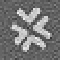
\includegraphics[height=\heightof{M}]{autanet.pdf}}
\definecolor{mygray}{gray}{0.333}
\iftypodisclaim%
\ifafour\newcommand\addprintnote{\begin{picture}(0,0)%
\put(245,149){\makebox(0,0){\rotatebox{90}{\tiny\color{mygray}\textsf{This
            document is designed for screen reading and
            two-up printing on A4 or Letter paper}}}}%
\end{picture}}% A4
\else\newcommand\addprintnote{\begin{picture}(0,0)%
\put(176,112){\makebox(0,0){\rotatebox{90}{\tiny\color{mygray}\textsf{This
            document is designed for screen reading and
            two-up printing on A4 or Letter paper}}}}%
\end{picture}}\fi%afourtrue
\makeoddfoot{plain}{}{\makebox[0pt]{\thepage}\addprintnote}{}
\else
\makeoddfoot{plain}{}{\makebox[0pt]{\thepage}}{}
\fi%typodisclaimtrue
\makeoddhead{plain}{\scriptsize\reporthead}{}{}
% \copypagestyle{manainitial}{plain}
% \makeheadrule{manainitial}{\headwidth}{0.5\normalrulethickness}
% \makeoddhead{manainitial}{%
% \footnotesize\sffamily%
% \scshape\headauthor}{}{\footnotesize\sffamily%
% \headtitle}
% \makeoddfoot{manaart}{}{\thepage}{}

\pagestyle{manaart}

\setlength{\droptitle}{-3.9\onelineskip}
\pretitle{\begin{center}\LARGE\sffamily%
\bfseries}
\posttitle{\bigskip\end{center}}

\makeatletter\newcommand*{\atf}{
\includegraphics[%trim=1pt 1pt 0pt 0pt,
totalheight=\heightof{@}]{atblack.png}}\makeatother
\providecommand{\affiliation}[1]{\textsl{\textsf{\footnotesize #1}}}
\providecommand{\epost}[1]{\texttt{\footnotesize\textless#1\textgreater}}
\providecommand{\email}[2]{\href{mailto:#1ZZ@#2 ((remove ZZ))}{#1\protect\atf#2}}

\preauthor{\vspace{-0.5\baselineskip}\begin{center}
\normalsize\sffamily%
\lineskip  0.5em}
\postauthor{\par\end{center}}
\predate{\DTMsetdatestyle{mydate}\begin{center}\footnotesize}
\postdate{\end{center}\vspace{-\medskipamount}}

\setfloatadjustment{figure}{\footnotesize}
\captiondelim{\quad}
\captionnamefont{\footnotesize\sffamily%
}
\captiontitlefont{\footnotesize}
%\firmlists*
\midsloppy
% handling orphan/widow lines, memman.pdf
% \clubpenalty=10000
% \widowpenalty=10000
% \raggedbottom
% Downes, memman.pdf
\clubpenalty=9996
\widowpenalty=9999
\brokenpenalty=4991
\predisplaypenalty=10000
\postdisplaypenalty=1549
\displaywidowpenalty=1602
\raggedbottom

\paragraphfootnotes%
%\setlength{\footmarkwidth}{1.3em}
% \threecolumnfootnotes
%\setlength{\footmarksep}{-\footmarkwidth}
%\setlength{\footparindent}{10em}
\footmarkstyle{\textsuperscript{%\color{myred}
\scriptsize\bfseries%\underline{
#1%}
}~}
%\footmarkstyle{\textsuperscript{\color{myred}\scriptsize\bfseries#1}~}
%\footmarkstyle{\textsuperscript{[#1]}~}

\selectlanguage{british}\frenchspacing

%%%%%%%%%%%%%%%%%%%%%%%%%%%%%%%%%%%%%%%%%%%%%%%%%%%%%%%%%%%%%%%%%%%%%%%%%%%%
%%% Paper's details
%%%%%%%%%%%%%%%%%%%%%%%%%%%%%%%%%%%%%%%%%%%%%%%%%%%%%%%%%%%%%%%%%%%%%%%%%%%%
\title{\propertitle}
\author{%
\hspace*{\stretch{1}}%
%% uncomment if additional authors present
% \parbox{0.5\linewidth}%\makebox[0pt][c]%
% {\protect\centering ***\\%
% \footnotesize\epost{\email{***}{***}}}%
% \hspace*{\stretch{1}}%
\parbox{0.75\linewidth}%\makebox[0pt][c]%
{\protect\centering P.G.L.  Porta Mana \href{https://orcid.org/0000-0002-6070-0784}{\protect
\includegraphics[scale=0.16]{orcid_32x32.png}}\\%
\footnotesize Kavli Institute, Trondheim\quad\epost{\email{piero.mana}{ntnu.no}}}%
\hspace*{\stretch{1}}%
}

%\date{Draft of \today\ (first drafted \firstdraft)}
\date{\firstpublished; updated \updated}

%%%%%%%%%%%%%%%%%%%%%%%%%%%%%%%%%%%%%%%%%%%%%%%%%%%%%%%%%%%%%%%%%%%%%%%%%%%%
%%% Macros @@@
%%%%%%%%%%%%%%%%%%%%%%%%%%%%%%%%%%%%%%%%%%%%%%%%%%%%%%%%%%%%%%%%%%%%%%%%%%%%

% Common ones - uncomment as needed
%\providecommand{\nequiv}{\not\equiv}
%\providecommand{\coloneqq}{\mathrel{\mathop:}=}
%\providecommand{\eqqcolon}{=\mathrel{\mathop:}}
%\providecommand{\varprod}{\prod}
\newcommand*{\de}{\partialup}%partial diff
\newcommand*{\pu}{\piup}%constant pi
\newcommand*{\delt}{\deltaup}%Kronecker, Dirac
%\newcommand*{\eps}{\varepsilonup}%Levi-Civita, Heaviside
%\newcommand*{\riem}{\zetaup}%Riemann zeta
%\providecommand{\degree}{\textdegree}% degree
%\newcommand*{\celsius}{\textcelsius}% degree Celsius
%\newcommand*{\micro}{\textmu}% degree Celsius
\newcommand*{\I}{\mathrm{i}}%imaginary unit
\newcommand*{\e}{\mathrm{e}}%Neper
\newcommand*{\di}{\mathrm{d}}%differential
%\newcommand*{\Di}{\mathrm{D}}%capital differential
%\newcommand*{\planckc}{\hslash}
%\newcommand*{\avogn}{N_{\textrm{A}}}
%\newcommand*{\NN}{\bm{\mathrm{N}}}
%\newcommand*{\ZZ}{\bm{\mathrm{Z}}}
%\newcommand*{\QQ}{\bm{\mathrm{Q}}}
\newcommand*{\RR}{\bm{\mathrm{R}}}
%\newcommand*{\CC}{\bm{\mathrm{C}}}
%\newcommand*{\nabl}{\bm{\nabla}}%nabla
%\DeclareMathOperator{\lb}{lb}%base 2 log
\DeclareMathOperator{\tr}{tr}%trace
%\DeclareMathOperator{\card}{card}%cardinality
%\DeclareMathOperator{\im}{Im}%im part
%\DeclareMathOperator{\re}{Re}%re part
%\DeclareMathOperator{\sgn}{sgn}%signum
%\DeclareMathOperator{\ent}{ent}%integer less or equal to
%\DeclareMathOperator{\Ord}{O}%same order as
%\DeclareMathOperator{\ord}{o}%lower order than
\newcommand*{\incr}{\triangle}%finite increment
\newcommand*{\defd}{\coloneqq}
\newcommand*{\defs}{\eqqcolon}
%\newcommand*{\Land}{\bigwedge}
%\newcommand*{\Lor}{\bigvee}
%\newcommand*{\lland}{\DOTSB\;\land\;}
%\newcommand*{\llor}{\DOTSB\;\lor\;}
%\newcommand*{\limplies}{\mathbin{\Rightarrow}}%implies
%\newcommand*{\suchthat}{\mid}%{\mathpunct{|}}%such that (eg in sets)
%\newcommand*{\with}{\colon}%with (list of indices)
%\newcommand*{\mul}{\times}%multiplication
%\newcommand*{\inn}{\cdot}%inner product
\newcommand*{\dotv}{\mathord{\,\cdot\,}}%variable place
%\newcommand*{\comp}{\circ}%composition of functions
%\newcommand*{\con}{\mathbin{:}}%scal prod of tensors
%\newcommand*{\equi}{\sim}%equivalent to 
\renewcommand*{\asymp}{\simeq}%equivalent to 
%\newcommand*{\corr}{\mathrel{\hat{=}}}%corresponds to
%\providecommand{\varparallel}{\ensuremath{\mathbin{/\mkern-7mu/}}}%parallel (tentative symbol)
\renewcommand*{\le}{\leqslant}%less or equal
\renewcommand*{\ge}{\geqslant}%greater or equal
\DeclarePairedDelimiter\clcl{[}{]}
%\DeclarePairedDelimiter\clop{[}{[}
%\DeclarePairedDelimiter\opcl{]}{]}
%\DeclarePairedDelimiter\opop{]}{[}
\DeclarePairedDelimiter\abs{\lvert}{\rvert}
%\DeclarePairedDelimiter\norm{\lVert}{\rVert}
\DeclarePairedDelimiter\set{\{}{\}}
%\DeclareMathOperator{\pr}{P}%probability
\newcommand*{\pf}{\mathrm{p}}%probability
\newcommand*{\p}{\mathrm{P}}%probability
%\newcommand*{\E}{\mathrm{E}}
%\renewcommand*{\|}{\nonscript\,\vert\nonscript\;\mathopen{}}
\renewcommand*{\|}[1][]{\nonscript\,#1\vert\nonscript\;\mathopen{}}
%\DeclarePairedDelimiterX{\cond}[2]{(}{)}{#1\nonscript\,\delimsize\vert\nonscript\;\mathopen{}#2}
%\DeclarePairedDelimiterX{\condt}[2]{[}{]}{#1\nonscript\,\delimsize\vert\nonscript\;\mathopen{}#2}
%\DeclarePairedDelimiterX{\conds}[2]{\{}{\}}{#1\nonscript\,\delimsize\vert\nonscript\;\mathopen{}#2}
%\newcommand*{\+}{\lor}
%\renewcommand{\*}{\land}
\newcommand*{\sect}{\S}% Sect.~
\newcommand*{\sects}{\S\S}% Sect.~
\newcommand*{\chap}{ch.}%
\newcommand*{\chaps}{chs}%
\newcommand*{\bref}{ref.}%
\newcommand*{\brefs}{refs}%
%\newcommand*{\fn}{fn}%
\newcommand*{\eqn}{eq.}%
\newcommand*{\eqns}{eqs}%
\newcommand*{\fig}{fig.}%
\newcommand*{\figs}{figs}%
\newcommand*{\vs}{{vs}}
%\newcommand*{\etc}{{etc.}}
%\newcommand*{\ie}{{i.e.}}
%\newcommand*{\ca}{{c.}}
\newcommand*{\eg}{{e.g.}}
\newcommand*{\foll}{{ff.}}
%\newcommand*{\viz}{{viz}}
\newcommand*{\cf}{{cf.}}
%\newcommand*{\Cf}{{Cf.}}
%\newcommand*{\vd}{{v.}}
\newcommand*{\etal}{{et al.}}
%\newcommand*{\etsim}{{et sim.}}
%\newcommand*{\ibid}{{ibid.}}
%\newcommand*{\sic}{{sic}}
%\newcommand*{\id}{\mathte{id}}%id matrix
%\newcommand*{\nbd}{\nobreakdash}%
%\newcommand*{\bd}{\hspace{0pt}}%
%\def\hy{-\penalty0\hskip0pt\relax}
\newcommand*{\labelbis}[1]{\tag*{(\ref{#1})$_\text{r}$}}
%\newcommand*{\mathbox}[2][.8]{\parbox[t]{#1\columnwidth}{#2}}
%\newcommand*{\zerob}[1]{\makebox[0pt][l]{#1}}
\newcommand*{\tprod}{\mathop{\textstyle\prod}\nolimits}
\newcommand*{\tsum}{\mathop{\textstyle\sum}\nolimits}
\newcommand*{\tint}{\begingroup\textstyle\int\endgroup\nolimits}
%\newcommand*{\tland}{\mathop{\textstyle\bigwedge}\nolimits}
%\newcommand*{\tlor}{\mathop{\textstyle\bigvee}\nolimits}
%\newcommand*{\sprod}{\mathop{\textstyle\prod}}
%\newcommand*{\ssum}{\mathop{\textstyle\sum}}
%\newcommand*{\sint}{\begingroup\textstyle\int\endgroup}
%\newcommand*{\sland}{\mathop{\textstyle\bigwedge}}
%\newcommand*{\slor}{\mathop{\textstyle\bigvee}}
\newcommand*{\T}{^\intercal}%transpose
%%\newcommand*{\QEM}%{\textnormal{$\Box$}}%{\ding{167}}
%\newcommand*{\qem}{\leavevmode\unskip\penalty9999 \hbox{}\nobreak\hfill
%\quad\hbox{\QEM}}

%%%%%%%%%%%%%%%%%%%%%%%%%%%%%%%%%%%%%%%%%%%%%%%%%%%%%%%%%%%%%%%%%%%%%%%%%%%%
%%% Custom macros for this file @@@
%%%%%%%%%%%%%%%%%%%%%%%%%%%%%%%%%%%%%%%%%%%%%%%%%%%%%%%%%%%%%%%%%%%%%%%%%%%%
 \definecolor{notecolour}{RGB}{68,170,153}
\newcommand*{\puzzle}{{\fontencoding{U}\fontfamily{fontawesometwo}\selectfont\symbol{225}}}
%\newcommand*{\puzzle}{\maltese}
\newcommand{\mynote}[1]{ {\color{notecolour}\puzzle\ #1}}
\newcommand*{\widebar}[1]{{\mkern1.5mu\skew{2}\overline{\mkern-1.5mu#1\mkern-1.5mu}\mkern 1.5mu}}

% \newcommand{\explanation}[4][t]{%\setlength{\tabcolsep}{-1ex}
% %\smash{
% \begin{tabular}[#1]{c}#2\\[0.5\jot]\rule{1pt}{#3}\\#4\end{tabular}}%}
% \newcommand*{\ptext}[1]{\text{\small #1}}
%\DeclareMathOperator*{\argsup}{arg\,sup}
% \newcommand*{\dob}{degree of belief}
% \newcommand*{\dobs}{degrees of belief}

\makeatletter
\newcommand*{\q}{}% Check if undefined
\DeclareRobustCommand*{\q}{%
  \mathbin{\mathpalette\bigcdot@{}}%
}
\newcommand*{\bigcdot@scalefactor}{0.75}
\newcommand*{\bigcdot@widthfactor}{1.5}
\newcommand*{\bigcdot@}[2]{%
  % #1: math style
  % #2: unused
  \sbox0{$#1\vcenter{}$}% math axis
  \sbox2{$#1\cdot\m@th$}%
  \hbox to \bigcdot@widthfactor\wd2{%
    \hfil
    \raise\ht0\hbox{%
      \scalebox{\bigcdot@scalefactor}{%
        \lower\ht0\hbox{$#1\bullet\m@th$}%
      }%
    }%
    \hfil
  }%
}
\makeatother


\newcommand*{\dime}{\clcl}
\newcommand*{\Un}{\textsf{1}}
\newcommand*{\Le}{\textsf{L}}
\newcommand*{\Ti}{\textsf{T}}
\newcommand*{\Ma}{\textsf{M}}
\newcommand*{\Te}{\Theta}
\newcommand*{\Cu}{\textsf{I}}
\newcommand*{\Fl}{\Phi}
\newcommand*{\En}{\Epsilon}%{\textsf{E}}
\newcommand*{\Xx}{\textsf{X}}
\newcommand*{\Yy}{\textsf{Y}}
\newcommand*{\Aa}{\textsf{A}}
\newcommand*{\Bb}{\textsf{B}}
\newcommand*{\Ss}{\textsf{S}}
\newcommand*{\Li}{\mathrm{L}}
\newcommand*{\ii}{\mathrm{i}}
%
\newcommand*{\yA}{\mathte{A}}
\newcommand*{\yB}{\mathte{B}}
\newcommand*{\yg}{\mathte{g}}
\newcommand*{\ygc}{\mathte{g}}
\newcommand*{\yT}{\mathte{T}}
\newcommand*{\yG}{\mathte{G}}
\newcommand*{\yR}{\mathte{R}}
\newcommand*{\yRi}{\mathte{Ric}}
\newcommand*{\ysc}{\rho}
\newcommand*{\yTo}{\bm{\tau}}
\newcommand*{\yom}{\bm{\omega}}
\newcommand*{\yta}{\bm{\tau}}
\newcommand*{\yv}{\bm{v}}
\newcommand*{\yu}{\bm{u}}
\newcommand*{\yw}{\bm{w}}
\renewcommand*{\i}{\indices}
\newcommand*{\dex}[1][i]{\frac{\de}{\de x^{#1}}}
\newcommand*{\dix}[1][i]{\di x^{#1}}
\newcommand*{\nab}{\nabla}
\newcommand*{\yGa}{\varGamma}
\newcommand*{\ds}{\mathit{ds}}
\newcommand*{\inct}{\incr t}
\newcommand*{\yCs}{\Bar{C}}
\newcommand*{\id}{\mathrm{id}}%id matrix
\newcommand*{\ye}{\bm{e}}
\newcommand*{\ygv}{\bm{\gamma}}
\newcommand*{\yt}{\bm{\sigma}}
\newcommand*{\yk}{\kappa}

%%% Custom macros end @@@

%%%%%%%%%%%%%%%%%%%%%%%%%%%%%%%%%%%%%%%%%%%%%%%%%%%%%%%%%%%%%%%%%%%%%%%%%%%%
%%% Beginning of document
%%%%%%%%%%%%%%%%%%%%%%%%%%%%%%%%%%%%%%%%%%%%%%%%%%%%%%%%%%%%%%%%%%%%%%%%%%%%
%\firmlists
\begin{document}
\captiondelim{\quad}\captionnamefont{\footnotesize}\captiontitlefont{\footnotesize}
\selectlanguage{british}\frenchspacing
\maketitle

%%%%%%%%%%%%%%%%%%%%%%%%%%%%%%%%%%%%%%%%%%%%%%%%%%%%%%%%%%%%%%%%%%%%%%%%%%%%
%%% Abstract
%%%%%%%%%%%%%%%%%%%%%%%%%%%%%%%%%%%%%%%%%%%%%%%%%%%%%%%%%%%%%%%%%%%%%%%%%%%%
\abstractrunin
\abslabeldelim{}
\renewcommand*{\abstractname}{}
\setlength{\absleftindent}{0pt}
\setlength{\absrightindent}{0pt}
\setlength{\abstitleskip}{-\absparindent}
\begin{abstract}\labelsep 0pt%
  \noindent This note illustrates how to perform dimensional analysis in
  general relativity and differential geometry, and tries to revive Dorgelo
  \amp\ Schouten's notion of \emph{absolute dimension} of a tensorial
  quantity. The absolute dimension is independent of the dimensions of the
  coordinate functions. The dimensional analysis of several important
  tensors and tensor operations is summarized. In particular it is shown
  that the components of a tensor need not have all the same dimension, and
  that the Riemann (once contravariant and trice covariant) and Ricci
  (fully covariant) tensors are dimensionless. The relation between
  dimension and operational meaning for the metric and
  stress-energy-momentum tensors is also
  discussed.
  % \\\noindent\emph{\footnotesize Note: Dear Reader \amp\ Peer,
  %   this manuscript is being peer-reviewed by you. Thank you.}
% \par%\\[\jot]
% \noindent
% {\footnotesize PACS: ***}\qquad%
% {\footnotesize MSC: ***}%
%\qquad{\footnotesize Keywords: ***}
\end{abstract}
\selectlanguage{british}\frenchspacing

%%%%%%%%%%%%%%%%%%%%%%%%%%%%%%%%%%%%%%%%%%%%%%%%%%%%%%%%%%%%%%%%%%%%%%%%%%%%
%%% Epigraph
%%%%%%%%%%%%%%%%%%%%%%%%%%%%%%%%%%%%%%%%%%%%%%%%%%%%%%%%%%%%%%%%%%%%%%%%%%%%
 \asudedication{\small For Emma}
% \vspace{\bigskipamount}
% \setlength{\epigraphwidth}{.7\columnwidth}
% %\epigraphposition{flushright}
% \epigraphtextposition{flushright}
% %\epigraphsourceposition{flushright}
% \epigraphfontsize{\footnotesize}
% \setlength{\epigraphrule}{0pt}
% %\setlength{\beforeepigraphskip}{0pt}
% %\setlength{\afterepigraphskip}{0pt}
% \epigraph{\emph{text}}{source}



%%%%%%%%%%%%%%%%%%%%%%%%%%%%%%%%%%%%%%%%%%%%%%%%%%%%%%%%%%%%%%%%%%%%%%%%%%%%
%%% BEGINNING OF MAIN TEXT
%%%%%%%%%%%%%%%%%%%%%%%%%%%%%%%%%%%%%%%%%%%%%%%%%%%%%%%%%%%%%%%%%%%%%%%%%%%%

\section{Introduction}
\label{sec:intro}


From the point of view of dimensional analysis, do all components of a
tensor need to have the same dimension? What is the dimension of the metric
and the curvature? And what is the dimension of the constant in the
Einstein equations?

There seem to be insecurity and incorrect notions, among some students and
even some researchers in relativity, regarding the dimensions of tensors
and of tensor components, the effect of tensor operators on dimensions, and
the dimension of constants in differential-geometric and field equations.
I've met, for example, with the statement that the components of a tensor
should all have the same dimension; and with calculations of the dimensions
of curvature tensors assuming that coordinates have dimensions of length.
That statement is wrong; and that assumption is unnecessary.

Several factors probably cause or contribute to such difficulties. Modern
texts in Lorentzian and general relativity commonly use geometrized units.
They say that, for finding the dimension of some constant in a tensorial
equation, it's sufficient to compare the dimensions of the tensors in the
equation. But this is not so immediate, because some tensors don't have
universally agreed dimensions -- prime example the metric tensor. Older
texts often use coordinates with dimension of length and time, and base
their dimensional analysis on that specific choice. They even multiply
coordinates with dimension of time, as well as some tensorial components,
by powers of $c$. They thus give the impression that coordinates ought to
always be lengths, and that all components of a tensor ought to have the
same dimension \citep[\eg][\sect~37 \eqn~(37.8)]{tolman1934_t1949}[\sect~32
\eqn~(32.15)]{landauetal1939_t1996}[\sect~10.1
\eqn~(10.15)]{adleretal1965_r1975}.

\medskip

The main purpose of this Note is to illustrate an extremely simple and
intuitive way of reasoning with which one can quickly and consistently
settle any dimensional-analysis questions in general relativity and
differential geometry; for example the dimension of the Riemann tensor, or
the dimensional results of contraction, of covariant derivative, of raising
an index. This way of reasoning is presented and illustrated in
\sects~\ref{sec:tensors}--\ref{sec:tensor_ops}. It's just an application of
the usual rules of dimensional analysis: if two quantities are summed, then
they must have the same dimension; the dimension of a product is the
product of the dimensions; and so on. This way of reasoning relies on the
coordinate-free, \emph{intrinsic} view of tensors and other
differential-geometrical objects, a brief reminder of which is given in
\sect~\ref{sec:remined}, with references.


Another important purpose of this Note is to revive the forgotten notion of
\emph{absolute dimension} of a tensor, and the distinction between it and
the dimensions of that tensor's \emph{components} in some coordinate
system. This notion is explained in \sect~\ref{sec:tensors}. The
absolute dimension, introduced by Schouten and Dorgelo
\citep{dorgeloetal1946}[\chap~VI]{schouten1951_r1989} and used in Truesdell
\amp\ Toupin \citep[Appendix II]{truesdelletal1960}, is invariant with respect to
the dimensions of the coordinates; it's an intrinsic property of a
tensor. The dimensions of the components depend instead on the dimensions
of the coordinate functions -- which can be completely arbitrary, as
discussed in \sect~\ref{sec:coords}. The absolute dimension should thus be
the primary focus in dimensional analysis in general relativity and in
differential geometry.




The rest of this Note is mainly an application of the intuitive way of
reasoning mentioned above and of the notion of absolute dimension. We'll
reveal and rectify a couple of misconceptions; for example, \emph{the
  components of a tensor need not have the same dimensions}. The results
for the main tensor operations and operators are summarized in
\sect~\ref{sec:tensor_ops}. The results for the curvature tensors and other
objects depending on a connection are presented in
\sect~\ref{sec:connection}. It is shown, in particular, that the absolute
dimension of the (contravariant and thrice covariant) Riemann and (fully
covariant) Ricci tensors is $\Un$, that is, they are dimensionless. Some
geometric objects or operators may be unfamiliar to researchers working in
general relativity only; their discussion may simply be skipped by these
readers.

The absolute dimension of the metric tensor is discussed in
\sect~\ref{sec:metric}. The literature on general relativity presents two
standard choices for it. The absolute dimension of the
stress-energy-momentum tensor is discussed in \sect~\ref{sec:stressenergy}.
The dimension of the constant in the Einstein equation is derived in
\sect~\ref{sec:einstein_eq}, and the two standard results from the
literature are recovered.

The final \sect~\ref{sec:summary} gives a summary of the main results, with
some additional comments.

\medskip

This Note assumes some familiarity with basic tensor calculus and related
notions, for example of co- and contravariance, symmetry and antisymmetry,
contraction. Some passages assume familiarity with the exterior calculus of
differential forms. Above all, familiarity with the intrinsic presentation
of differential geometry is assumed; but the general ideas should be
understandable even without such familiarity. The notation used here is
briefly presented in \sect~\ref{sec:notation}.

Finally, quoting Truesdell \amp\ Toupin \citep[Appendix \sect~7
footnote~4]{truesdelletal1960}, \enquote{dimensional analysis remains a
  controversial and somewhat obscure subject. We do not attempt a complete
  presentation here.}


% \citep{aldersley1977} also confuses component- and absolute dimensions

\section{Notation}
\label{sec:notation}

For the notation in dimensional analysis I use \textsc{iso} conventions:
$\dim(\yA)$ is the dimension of the quantity $\yA$, and among the base
quantities are mass $\Ma$, length $\Le$, time $\Ti$, temperature $\Te$,
electric current $\Cu$. Note that I don't discuss \emph{units} -- it
doesn't matter here whether the unit for length is the metre or the
centimetre, for example.

Since the type of a tensor -- that is, the number and ordering of its
covariant and contravariant \enquote{slots}
\citep[\sect~3.2]{misneretal1970_r1973} -- is important in dimensional
analysis, I often denote it explicitly with a notation like
$\yA\i{_{\q}^{\q\q}}$ to indicate that $\yA$ is covariant in its first slot
and contravariant in its second and third slots. Its components would thus
be $(A\i{_{i}^{jk}})$. For brevity I'll call this a
\enquote{co-contra-contravariant} tensor, with an obvious naming
generalization for other types. In spirit this notation is similar to the
abstract-index one of Penrose \amp\ Rindler
\citep[\sect~2.2]{penroseetal1984_r2003}; but I avoid using letters for the
indices, so that the notational difference between a tensor and its
components, which is very important for our discussion, doesn't disappear.

I denote the contraction of the $\alpha$th and $\beta$th slots (which must
have opposite variant types) of a tensor $\yA$ by $\tr_{\alpha\beta}\yA$,
and the transposition (swapping) of the $\alpha$th and $\beta$th slots with
$\yA^{\intercal_{\alpha\beta}}$. In index notation these operations are
  \begin{equation*}
    A\i{_{\dotsm\;}^{%
      \overset{\mathclap{\scriptstyle\text{$\alpha$th slot}}}{i}
    }_{\dotsm\;%
      \underset{\mathclap{\scriptstyle\text{$\beta$th slot}}}{i}
      \;\dotsm}}
  \qquad\text{and}\qquad
      A\i{_{\dotsm\;}^{%
      \overset{\mathclap{\scriptstyle\text{$\alpha$th slot}}}{i}
    }_{\dotsm\;%
      \underset{\mathclap{\scriptstyle\text{$\beta$th slot}}}{j}
      \;\dotsm}}
  \mapsto
  A\i{_{\dotsm\;%
      \underset{\mathclap{\scriptstyle\text{$\alpha$th slot}}}{j}
    \;\dotsm\;}^{%
      \overset{\mathclap{\scriptstyle\text{$\beta$th slot}}}{i}
      }_{\;\dotsm}}.
  \end{equation*}

  % $\yA\i{^{\q \mathrm{c}}_{\q \mathrm{c}\q}}$



\section{Intrinsic view of differential-geometric objects:  brief
  reminder}
\label{sec:remined}


From the intrinsic point of view, a tensor is defined by its geometric
properties. For example, a vector field $\yv \equiv \yv(\dotv)$ is an
object that operates on functions defined on the (spacetime) manifold,
yielding new functions, with the properties $\yv(af+bg)=a\yv(f)+b\yv(g)$
and $\yv(fg)=\yv(f)g+f\yv(g)$ for all functions $f$, $g$ and reals $a$,
$b$. A covector field (1-form) $\yom$ is an object that operates on vector
fields, yielding functions (\enquote{duality}), with the property
$\yom(f\yu+g\yv)=f\yom(\yu)+g\yom(\yv)$ for all vector fields $\yu$, $\yv$
and functions $f$, $g$. The sum of vector or covector fields, and their
products by functions -- let's call this \enquote{linearity} -- are defined
in an obvious way. Tensors are constructed from these objects.

A system of coordinates $(x^{i})$ is just a set of linearly independent
functions. This set gives rise to a set of vectors fields
$\Bigl(\dex\Bigr)$ and to a set of covector fields $(\dix)$ by the obvious
requirements that $\dex(x^{j})=\delt\i{_{i}^{j}}$ and
$\dix\Bigl(\dex[j]\Bigr)=\delt\i{^{i}_{j}}$. These two sets can be used as bases
to express all other vectors and covectors as linear combinations. A
vector field $\yv$ can thus be written as
\begin{equation}
  \label{eq:vector_intrinsic}
  \yv \equiv \sum_{i}v^{i}\dex \equiv v^{i}\dex ,
\end{equation}
where the \emph{functions} $v^{i}\defd \yv(x^{i})$ are its components with
respect to the basis $\Bigl(\dex\Bigr)$. Analogously for a covector field.

\medskip

For the presentation of the intrinsic view I recommend the excellent texts
by Choquet-Bruhat \etal\ \citey{choquetbruhatetal1977_r1996}, Boothby
\citey{boothby1975_r2003}, Abraham \etal\ \citey{abrahametal1983_r1988},
Bossavit \citey{bossavit1991}, Burke
\citey{burke1985_r1987}[\chap~2]{burke1980b}, and more on the
general-relativity side Misner \etal\
\citey[\chap~9]{misneretal1970_r1973}, Gourgoulhon
\citey[\chap~2]{gourgoulhon2007_r2012}, Penrose \amp\ Rindler
\citey[\chap~4]{penroseetal1984_r2003}. \textcolor{white}{If you find this
  you can claim a postcard from me.}


% \mynote{check \citep{fischeretal1972}}
 

\section{Coordinates}
\label{sec:coords}

From a physical point of view, a coordinate is just a function that
associates a value of a physical quantity with every event in a region (the
domain of the coordinate chart) of spacetime. Together with the other
coordinates, such function allows us to uniquely identify every event
within that region. Any physical quantity will do: the distance from
something, the time elapsed since something, an angle, an energy density,
the strength of a magnetic flux, a temperature, and so on. A coordinate can
thus have any dimension: length $\Le$, time $\Ti$, angle $\Un$, energy
density $\En \defd \Ma\Le^{-1}\Ti^{-2}$, magnetic flux
$\Fl \defd \Ma\Le^{2}\Ti^{-2}\Cu^{-1}$, temperature $\Te$, and so on.

The functional relation between two sets of coordinates must of course be
dimensionally consistent. For example, if $\dim(x^{0})=\Ti$ and
$\dim(x^{1})=\Le$, and we introduce a coordinate $\xi(x^{0},x^{1})$ with
dimension $\Un$, additive in the previous two, then we must have
$\xi = a x^{0} + bx^{1}$ with $\dim(a)=\Ti^{-1}$ and $\dim(b)=\Le^{-1}$.

%The dimensions of the coordinates don't matter, as we'll now see.

\section{Tensors: absolute dimension and components' dimensions}
\label{sec:tensors}

Consider a system of coordinates $(x^i)$ with dimensions $(\Xx_i)$, and the
ensuing sets of covector fields (1-forms) $\dix$ and of vector fields
$\Bigl(\dex\Bigr)$, bases for the cotangent and tangent spaces. Their
tensor products are bases for the tangent spaces of higher tensor types.

The differential $\dix$ traditionally has the same dimension as $x^{i}$:
$\dim(\dix) = \Xx_{i}$, and the vector $\dex$ traditionally has the
inverse dimension: $\dim\dex = {\Xx_{i}}^{-1}$. % We'll see later that these
% conventions are self-consistent.

For our discussion let's take a concrete example: a contra-covariant tensor
field $\yA \equiv \yA\i{^{\q}_{\q}}$. The discussion generalizes to tensors
of other types in an obvious way.

The tensor $\yA$ can be expanded in terms of the basis vectors and
covectors, as mentioned in \sect~\ref{sec:remined}:
\begin{equation}
  \label{eq:expansion_tensor}
  \yA = A\i{^{i}_{j}}\, \dex\otimes\dix[j]
  \equiv A\i{^{0}_{0}}\,\dex[0]\otimes\dix[0] + 
  A\i{^{0}_{1}}\,\dex[0]\otimes\dix[1] + \dotsb {}.
\end{equation}
Each function
\begin{equation}
  A\i{^{i}_{j}} \defd  \yA\Bigl(\dix, \dex[j]\Bigr)
  \label{eq:components_def}
\end{equation}
is a \emph{component} of the tensor in this coordinate system.

\medskip

To make dimensional sense, all terms in the sum~\eqref{eq:expansion_tensor}
must have the same dimension. This is possible only if the generic
component $A\i{^{i}_{j}}$ has dimension
\begin{equation}
  \label{eq:dim_component}
  \dim\bigl(A\i{^{i}_{j}}\bigr) = \Aa\;{\Xx_{i}}\,{\Xx_{j}}^{-1},
\end{equation}
where $\Aa$ is \emph{common} to all components. In fact, the
${\Xx_{i}}\,{\Xx_{j}}^{-1}$ term cancels the ${\Xx_{i}}^{-1}\,{\Xx_{j}}$
term coming from $\dex\otimes\dix[j]$ in the
sum~\eqref{eq:expansion_tensor}, and each summand therefore has dimension
$\Aa$.

The generalization of the formula above to tensors of other types is obvious:
\begin{multline}
  \label{eq:dim_component_generic}
  \dim\bigl(A\i{^{ij\dotso}_{kl\dotso}}\bigr) = \Aa\;{\Xx_{i}}\,{\Xx_{j}}\dotsm\,
  {\Xx_{k}}^{-1}\,{\Xx_{l}}^{-1}\dotsm,
  \\
  \text{where the ordering of the indices doesn't matter.}
\end{multline}

For example, if  we're using coordinates with dimensions
\begin{equation}
  \label{eq:example_coords}
  \dim(x^{0})=\Te,\quad
  \dim(x^{1})=\Le,\quad
  \dim(x^{2})=\Le,\quad
  \dim(x^{3})=\Ma\Le^{-1}\Ti^{-2},
\end{equation}
then the components of $\yA$ have dimensions
\begin{equation}
  \label{eq:example_components}
  \Bigl(\dim\bigl(A\i{^{i}_{j}}\bigr)\Bigr) =
 \Aa\times \begin{pmatrix}
   \Un & \Le^{-1}\Te & \Le^{-1}\Te & \Ma^{-1}\Le\Ti^{2}\Te
   \\
   \Le\Te^{-1} & \Un & \Un & \Ma^{-1}\Le^{2}\Ti^{2}
   \\
   \Le\Te^{-1} & \Un & \Un & \Ma^{-1}\Le^{2}\Ti^{2}
   \\
   \Ma\Le^{-1}\Ti^{-2}\Te^{-1} & \Ma\Le^{-2}\Ti^{-2} & \Ma\Le^{-2}\Ti^{-2} & \Un
  \end{pmatrix}.
\end{equation}
Clearly most components have different dimensions. But this doesn't matter.
What matters is that the sum~\eqref{eq:expansion_tensor} be dimensionally
consistent. (Fokker \citep[\sect~VII.1 p.~88]{fokker1960_t1965}, for
example, uses a metric tensor with components having different dimensions.)

\medskip

The dimension $\Aa$, which is also the final dimension of the
sum~\eqref{eq:expansion_tensor}, is called the \emph{absolute dimension}
\citep{dorgeloetal1946}[\chap~VI]{schouten1951_r1989} of the tensor $\yA$,
and we write
\begin{equation}
  \label{eq:abs_dim}
  \dim(\yA) = \Aa.
\end{equation}
This is the intrinsic dimension of the tensor, independent of any
coordinate system. It reflects the physical or operational
\citep{bridgman1927_r1958}[see
also][\sect~A.2]{synge1960}[\sects~A.3--4]{truesdelletal1960} meaning of
the tensor. We'll see an example of what this mean in
\sect~\ref{sec:metric} with the metric tensor.


\medskip

Different coordinate systems lead to different dimensions of the
\emph{components} of a tensor $\yA$, but the absolute dimension of the
tensor remains the same. Formula~\eqref{eq:dim_component_generic} for the
dimensions of the components is consistent under changes of coordinates.
For example, in new coordinates $({x}^{i'})$ with dimensions
$({\Xx}_{i'})$, the new components of $\yA$ are
\begin{equation}
  \label{eq:coords_change}
  {A}\i{^{i'}_{j'}} = A\i{^{i}_{j}}
  \,\frac{\de {x}^{i'}}{\de x^{i}}
  \,\frac{\de {x}^{j}}{\de {x}^{i'}}
\end{equation}
and a quick check shows that
$\dim({A}\i{^{i'}_{j'}}) = \Aa\,{\Xx}_{i'}\,{{\Xx}_{j'}}^{-1}$, consistent
with the general formula~\eqref{eq:dim_component_generic}. % (You may have noticed
% that the partial-derivative symbol $\de$ is not in boldface in the last
% expression; that's on purpose but I won't dwell on the reason here, because
% it doesn't affect our discussion.)

\smallskip

In the following I'll drop the adjective
\enquote{absolute} when it's clear from the context.

\section{Tensor operations}
\label{sec:tensor_ops}

By the reasoning of the previous section, which simply applies standard
dimensional considerations to the basis
expansion~\eqref{eq:expansion_tensor}, it's easy to find the resulting
absolute dimension of various operations and operators on tensors and
tensor fields.

Here is a summary of the dimensional rules for the main
differential-geometric operations and operators, except for the covariant
derivative, the metric, and related tensors, discussed more in depth in
\sects~\ref{sec:connection}--\ref{sec:metric} below. Some of these rules
are really definition or conventions, as briefly discussed in their
description. The others can be proved; I only give a proof for one of them,
leaving the other proofs as an exercise. For reference, in brackets I give
the section of Choquet-Bruhat \etal\ \citey{choquetbruhatetal1977_r1996}
where these operations are defined.


\begin{itemize}[wide=0pt]
\item The \emph{tensor product} [III.B.5] multiplies dimensions:
  \begin{equation}
  \dim(\yA\otimes\yB) = \dim(\yA)\dim(\yB).\label{eq:tensor_mult}
\end{equation}

This is actually a definition or convention. In fact we tacitly used this
rule already in \sect~\ref{sec:tensors} for the tensors
$\dex\otimes\dix[j]$ in the coordinate
expansion~\eqref{eq:expansion_tensor}. It is a natural definition, because
for tensors of order 0 -- that is, functions -- the tensor product is just
ordinary multiplication, and the dimension of a product is the product of
the dimensions. And it is a definition that doesn't lead to
inconsistencies.

% Consider for example the tensor product of $\yA\i{^{\q}_{\q}}$ and
% $\yB\i{_{\q\q}^{\q}}$. It introducing coordinates $(x^{i})$ and their
% related basis vectors and covectors, it can be written as the sum
% \begin{equation}
%   \label{eq:tensor_prod_example}
%   \yA \otimes \yB =
%   A\i{^{i}_{j}}\,B\i{_{kl}^{m}}\;
%   \dex[i]\otimes\dix[j]\otimes\dix[k]\otimes\dix[l]\otimes\dex[m].
% \end{equation}
% Equating the dimensions of the left and right sides, and considering that
% \begin{equation}\label{eq:dim_A_and_B}
%   \dim(A\i{^{i}_{j}})= \dim(\yA)\,\Xx_{i}\,{\Xx_{j}}^{-1},
%   \quad
%   \dim(B\i{_{kl}^{m}})= \dim(\yB)\,{\Xx_{k}}^{-1}\,{\Xx_{l}}^{-1}\,\Xx_{m},
% \end{equation}
% owing to the generalization of the formula for the
% components~\eqref{eq:dim_component_generic}, we find that all $\Xx$ terms cancel
% out, leaving the result~\eqref{eq:tensor_mult}.

% \smallskip

% from which it follows that
% \begin{equation}
%   \label{eq:dim_comp_tensor_prod}
%   \dim(A\i{^{i}_{j}}\,B\i{_{kl}^{m}}) =
%   \Aa\,\Bb\;
%   \Xx_{i}\,{\Xx_{j}}^{-1}\,{\Xx_{k}}^{-1}\,{\Xx_{l}}^{-1}\,\Xx_{m}
% \end{equation}
% with $\Aa = \dim(\yA)$ and $\Bb = \dim(\yB)$. Comparing with the
% generalization of the formula for the components~\eqref{eq:dim_component_generic},
% we see that the absolute dimension of $\yA\otimes\yB$ is therefore
% $\Aa\Bb \equiv \dim(\yA)\,\dim(\yB)$.



\item The \emph{contraction} [III.B.5] or trace of the $\alpha$th and $\beta$th
  slots of a tensor has the same dimension as the tensor:
  \begin{equation}
    \dim(\tr_{\alpha\beta}\yA) = \dim(\yA).
    \label{eq:tensor_contr}
  \end{equation}
  Note that the formula above only holds \emph{without}
  raising or lowering indices; see \sect~\ref{sec:metric} for those
  operations.

  This operation can be traced back to the duality of vectors and covectors
  mentioned in \sect~\ref{sec:remined}: a covector field $\yom$ operates
  linearly on a vector field $\yv$ to yield a function $f=\yom(\yv)$. Also
  in this case we have that $\dim(f)=\dim(\yom)\dim(\yv)$ by definition or
  convention, and the rule~\eqref{eq:tensor_contr} follows from this
  convention. Also in this case this convention seems very natural, owing
  to the linearity properties of the trace, and doesn't lead to
  inconsistencies.

  

\item The \emph{transposition} (called \enquote{building an isomer} by
  Schouten \citep[\sect~I.3 p.~13]{schouten1924_r1954}[\sect~II.4
  p.~20]{schouten1951_r1989}) of the $\alpha$th and $\beta$th slots of a
  tensor has the same dimension as the tensor:
  \begin{equation}
    \dim(\yA^{\intercal_{\alpha\beta}}) = \dim(\yA).
    \label{eq:tensor_transp}
  \end{equation}


\item The \emph{Lie bracket} [III.B.3] of two vectors has the product of their dimensions:
  \begin{equation}
    \dim(\clcl{\yu,\yv}) =\dim(\yu)\dim(\yv).
    \label{eq:lie_bracket}
\end{equation}

In fact, in coordinates $(x^{i})$ the bracket can be expressed as
\begin{equation}
  \label{eq:bracket_coords}
  \clcl{\yu,\yv} =
  \biggl( u\i{^{j}}\frac{\de v\i{^{i}}}{\de x\i{^{j}}}
  - v\i{^{j}}\frac{\de u\i{^{i}}}{\de x\i{^{j}}} \biggr)\;\dex,
\end{equation}
and equating the dimensions of the left and right side, considering that
\begin{equation}
  \label{eq:dim_u_and_v}
  \dim(u\i{^{i}}) = \dim(\yu)\,\Xx_{i},\quad
  \dim(v\i{^{i}}) = \dim(\yv)\,\Xx_{i},
\end{equation}
we find again that all $\Xx$ terms cancel out leaving the
result~\eqref{eq:lie_bracket}.

\smallskip


% \item The \emph{pull-back} and \emph{push-forward} of a map $F$ between
%   manifolds don't change the dimensions of the tensors they map.
%   \begin{equation}
%   \dim(\yA\otimes\yB) = \dim(\yA)\dim(\yB).\label{eq:tensor_mult}
% \end{equation}

\item The \emph{Lie derivative} [III.C.2] of a tensor with respect to a
  vector field has the product of the dimensions of the tensor and of the
  vector:
  \begin{equation}
    \dim(\Li_{\yv}\yA) =\dim(\yv)\dim(\yA).
    \label{eq:lie_der}
\end{equation}
\end{itemize}

\medskip

Regarding operations and operators on differential forms:

\begin{itemize}[wide=0pt]
\item The \emph{exterior product} [IV.A.1] of two differential forms
  multiplies their dimensions:
  \begin{equation}
  \dim(\yom\land\yta) = \dim(\yom)\dim(\yta).\label{eq:ext_prod}
\end{equation}
  
\item The \emph{interior product} [IV.A.4] of a vector and a form
  multiplies their dimensions:
  \begin{equation}
    \dim(\ii_{\yv}\yom) =\dim(\yv)\dim(\yom).
    \label{eq:inter_prod}
\end{equation}

\item The \emph{exterior derivative} [IV.A.2] of a form has the same
  dimension of the form:
  \begin{equation}
    \dim(\di\yom) =\dim(\yom).
    \label{eq:ext_deriv}
  \end{equation}
  This can be proven using the identity
  $\di\,\ii_{\yv}+\ii_{\yv}\,\di = \Li_{\yv}$ or similar identities
  \citep[\chap~9 p.~180 Theorem~9.78]{curtisetal1985}[\sect~6.4
  Theorem~6.4.8]{abrahametal1983_r1988} together with
  \eqns~\eqref{eq:lie_der} and~\eqref{eq:inter_prod}.

\item The \emph{integral} [IV.B.1] of a form over a submanifold has the
  same dimension as the form:
  \begin{equation}
    \dim\bigl(\tint_{c}\yom\bigr) =\dim(\yom).
    \label{eq:integration}
  \end{equation}
\end{itemize}

% \medskip

% The resultant absolute dimensions of other operators, for example the
% determinant \citep[\sect~6.2]{abrahametal1983_r1988}, can be obtained by
% similar reasoning.

\section{Curves and integral curves}
\label{sec:curves}


Consider a curve into spacetime, $C\colon s \mapsto P(s)$, with the
parameter $s$ having dimension $\dim(s)=\Ss$.


If we consider the events of the spacetime manifold as dimensionless
quantities, then the dimension of the tangent or velocity vector $\dot{C}$
to the curve is
\begin{equation}
  \label{eq:dim_velocity}
  \dim(\dot{C}) = \Ss^{-1},
\end{equation}
owing to the definition
\citep[\sect~III.B.1]{choquetbruhatetal1977_r1996}[\sect~IV.(1.9)]{boothby1975_r2003}
\begin{equation}
  \label{eq:def_tangent_curve}
\dot{C} \defd \frac{\de x^{i}[C(s)]}{\de s}\;\dex .
\end{equation}
% or considering that $\dot{C}$ can be interpreted as the push-forward of
% $\partial_s$, that is, $C_*(\partial_s)$.

This has a quirky but interesting consequence. Given a vector field $\yv$
we say that $C$ is an integral curve for it if
\begin{equation}
  \yv = \dot{C}
  \label{eq:integral_curve}
\end{equation}
(or more precisely $\yv_{C(s)} = \dot{C}_{C(s)}$ in usual
differential-geometric notation
\citep[\sect~III.B.1]{choquetbruhatetal1977_r1996}) at all events $C(s)$ in
the image of the curve. From the point of view of dimensional analysis this
definition can only be valid if $\yv$ has dimension $\Ss^{-1}$. If $\yv$
and $s^{-1}$ have different dimensions -- a case which can happen for
physical reasons -- the condition~\eqref{eq:def_tangent_curve} must be
modified into $\yv = k\dot{C}$, where $k$ is a possibly dimensionful
constant. This is equivalent to considering an affine and dimensional
reparameterization of $C$.


\section{Connection, covariant derivative, curvature tensors}
\label{sec:connection}

Consider an arbitrary connection
\citep[\sect~V.B]{choquetbruhatetal1977_r1996} with covariant derivative
$\nab$. For the moment we don't assume the presence of any metric
structure.

The covariant derivative of the product $f\yv$ of a function and a vector
satisfies \citep[\sect~V.B.1]{choquetbruhatetal1977_r1996}
\begin{equation}
  \label{eq:basic_property_covder}
  \nab(f\yv) = \di f \otimes \yv + f\nab\yv.
\end{equation}
The first summand, from formulae~\eqref{eq:ext_deriv}
and~\eqref{eq:tensor_mult}, has dimension $\dim(f)\dim(\yv)$; for
dimensional consistency this must also be the dimension of the second
summand. Thus
\begin{equation}
  \label{eq:dim_cov_der_vect}
  \dim(\nab\yv) = \dim(\yv).
\end{equation}
It follows that the \emph{directional} covariant derivative $\nab_{\yu}$
has dimension
\begin{equation}
  \label{eq:dim_dircov_der_vect}
  \dim(\nab_{\yu}\yv) = \dim(\yu)\dim(\yv),
\end{equation}
and by its derivation properties \citep[\sect~V.B.1
p.~303]{choquetbruhatetal1977_r1996} we see that
formula~\eqref{eq:dim_cov_der_vect} extends from vectors to 
tensors of arbitrary type.

\medskip

In the coordinate system $(x^{i})$, the action of the covariant derivative
is carried by the \emph{connection coefficients} or Christoffel symbols
$(\yGa\i{^{i}_{jk}})$ defined by
\begin{equation}
  \label{eq:christoffel}
  \nab\dex[k] = \yGa\i{^{i}_{jk}}\; \dix[j]\otimes\dex[i].
\end{equation}
From this equation and the previous ones it follows that these coefficients
have dimensions
\begin{equation}
  \label{eq:dim_christoffel}
  \dim(\yGa\i{^{i}_{jk}}) = \Xx_{i}\, {\Xx_{j}}^{-1}\,{\Xx_{k}}^{-1}.
\end{equation}

\medskip

The \emph{torsion} $\yTo\i{^{\q}_{\q\q}}$, \emph{Riemann
  curvature} $\yR\i{^{\q}_{\q\q\q}}$, and \emph{Ricci
  curvature} $\yRi\i{_{\q\q}}$ tensors are defined by
\citep[\sect~V.B.1]{choquetbruhatetal1977_r1996}
\begin{gather}
  \label{eq:torsion_eq}
\yTo(\yu,\yv) \defd \nab_{\yu}\yv - \nab_{\yv}\yu - \clcl{\yu,\yv},
\\
\yR(\yu,\yv;\yw) \defd
\nab_{\yu}\nab_{\yv}\yw - \nab_{\yv}\nab_{\yu}\yw
- \nab_{\clcl{\yu,\yv}}\yw,
  \label{eq:riemann_eq}  
\\
\yRi\i{_{\q\q}} \defd \tr_{13} \yR\i{^{\q}_{\q\q\q}} \;.
  \label{eq:ricci_eq}  
\end{gather}
From these definitions and the results of \sect~\ref{sec:tensor_ops} we
find the dimensional requirements
\begin{gather}
  \label{eq:torsion_eq_dim}
\dim(\yTo\i{^{\q}_{\q\q}})\dim(\yu)\dim(\yv) = \dim(\yu) \dim(\yv),
\\
\dim(\yR\i{^{\q}_{\q\q\q}})\dim(\yu)\dim(\yv)\dim(\yw) =
\dim(\yu)\dim(\yv)\dim(\yw),
\label{eq:riemann_eq_dim}
\\
\dim(\yRi\i{_{\q\q}}) = \dim(\yR\i{^{\q}_{\q\q\q}}),
  \label{eq:ricci_eq_dim}  
\end{gather}
which imply that \emph{torsion, Riemann curvature, and Ricci curvature are
  dimensionless}:
\begin{equation}
  \label{eq:dim_torsion_riemann_ricci}
  \dim(\yTo\i{^{\q}_{\q\q}}) =
  % \label{eq:dim_riem}
   \dim(\yR\i{^{\q}_{\q\q\q}}) =
  % \label{eq:dim_ricci}
   \dim(\yRi\i{_{\q\q}}) =\Un.
\end{equation}
The exact contra- and covariant type used above for these tensors is very
important in these equations. If we raise any of their indices using a
metric, their dimensions will generally change.

Misner \etal\ \citey[pp.~35, 407]{misneretal1970_r1973} say that
\enquote{curvature}, the Riemann or Einstein tensors (for which see
\sect~\ref{sec:metric} below), has dimension $\Le^{-2}$, a statement
seemingly at variance with the dimensionless
results~\eqref{eq:dim_torsion_riemann_ricci}. But I believe that they refer
to the \emph{components} of those tensors, in specific coordinates of
dimension $\Le$, and using geometrized units. In such specific coordinates
every \emph{component} $R\i{^{i}_{jkl}}$ does indeed have dimension
$\Le^{-2}$, according to the general formula~\eqref{eq:dim_component_generic}, if
and only if the \emph{absolute} dimension of $\yR$ is unity,
$\dim(\yR)=\Un$. So I believe that there's no real contradiction with
Mister \etal's statement and the
results~\eqref{eq:dim_torsion_riemann_ricci}. This possible
misunderstanding shows that it's important to distinguish between absolute
dimensions, which don't depend on any specific coordinate choice, and
component dimensions, which do.

\medskip

The formulae above are also valid if a metric is defined and the connection
is compatible with it. The connection coefficients in this case are defined
in terms of the metric tensor, but using the results of
\sect~\ref{sec:metric} it's easy to see that
\eqns~\eqref{eq:dim_cov_der_vect}, \eqref{eq:dim_dircov_der_vect},
\eqref{eq:dim_christoffel}, \eqref{eq:dim_torsion_riemann_ricci} still
hold.


\section{Metric and related tensors and operations}
\label{sec:metric}

Let's now consider a metric tensor $\yg\i{_{\q\q}}$. What is its absolute
dimension $\dim(\yg)$? There seem to be two choices in the literature; both
can be derived from the operational meaning of the metric.


Consider a (timelike) worldline $s \mapsto C(s)$, $s\in \clcl{a,b}$,
between events $C(a)$ and $C(b)$. The metric tells us the \emph{proper
  time} $\inct$ elapsed for an observer having that worldline, according to
the formula
%\begin{subequations}\label{eq:dimg_t}\tag{(\ref{eq:dimg_t})}
\begin{equation}%\addtocounter{equation}{1}\tag{\theequation a}
  \label{eq:proper_time}
\inct =  \int_a^b\!\!\!\di s\;
\sqrt{\abs*{\yg[\dot{C}(s),\dot{C}(s)]}}.
\end{equation}
From the results of \sect~\ref{sec:tensor_ops} this formula implies that
%\begin{equation}
%  \label{eq:dim_dt}
 $\Ti \equiv \dim(\inct) = \sqrt{\dim(\yg\i{_{\q\q}})}$,
%\end{equation}
(independently of the dimension of $s$) and therefore
\begin{equation}%\addtocounter{equation}{1}\tag{\theequation a}
    \label{eq:dim_g}
    \dim(\yg\i{_{\q\q}}) = \Ti^{2}.
  \end{equation}
%\end{subequations}

  Many authors \citep[\eg][\sect~V.62
  \eqn~(62.02)]{fock1955_t1964}[\chap~11
  \eqn~(11.21)]{curtisetal1985}[\sect~5.3
  \eqn~(5.6)]{rindler1969_r1986}[\chap~6 \eqn~(6.24)]{hartle2003}, however,
  prefer to include a dimensional factor $1/c$ in front of the
  integral~\eqref{eq:proper_time}:
\begin{equation}%\addtocounter{equation}{-1}\tag{\theequation b}
  \label{eq:proper_time_c}
  \inct = \frac{1}{c} \int_a^b\!\!\!\di s\;
  \sqrt{\abs*{\ygc[\dot{C}(s),\dot{C}(s)]}},
\end{equation}
thus obtaining
\begin{equation}%\addtocounter{equation}{1}\tag{\theequation b}
  \label{eq:dim_g_c}
  \dim(\ygc\i{_{\q\q}}) = \Le^{2}.
\end{equation}
%To avoid confusion I'm using $\ygc$ for the metric with such dimension.

The choice~\eqref{eq:dim_g_c} seems also supported by the traditional
expression for the \enquote{line element $\ds^{2}$} as it appears in many
works (for an exception, with dimension $\Ti^{2}$, see Kilmister
\citep[\chap~II p.~25]{kilmister1973}{kilmister1973}),
\begin{equation}
  \label{eq:line_elem}
  \ds^{2} = c^2\mathit{dt}^2 - \mathit{dx}^2 -\mathit{dy}^2 - \mathit{dz}^2,
\end{equation}
possibly with opposite signature. If the
coordinates $(t,x,y,z)$ have the dimensions suggested by their symbols,
this formula has dimension $\Le^{2}$, so that if we interpret
\enquote{$\ds^{2}$} as $\ygc$ we find $\dim(\ygc) = \Le^{2}$. The
line-element expression above often has an ambiguous differential-geometric
meaning, however, because it may represent \emph{the metric applied to some
  unspecified vector}, that is, $\yg(\yv,\yv)$, where $\yv$ is left
unspecified \citep[\cf][Box~3.2~D p.~77]{misneretal1970_r1973}. In this
case we have
\begin{equation}
  \label{eq:line_elem_dim_ambiguous}
  \Le^{2} = \dim(\yg)\dim(\yv)^{2}
\end{equation}
and the dimension of $\yg$ is ambiguous.%  -- possibly dimensionless if $\yv$
% has dimension of length, but we'll see in \sect~\ref{sec:einstein_eq} that
% a dimensionless $\yg$ isn't quite compatible with the Einstein equation.

\medskip

The standard choices for $\dim{\yg}$ are thus $\Ti^{2}$ or $\Le^{2}$. My
favourite choice is the first, \eqref{eq:dim_g}, for reasons discussed by
Synge and Bressan \citep[\sects~III.2--4]{synge1960b}[\sects~15,
18]{bressan1978}. Synge gives a vivid summary: \citep[\sect~III.3
pp.~108--109]{synge1960b}
\begin{quote}\footnotesize
  We are now launched on the task of giving physical meaning to the
  Riemannian geometry \textelp{}. It is indeed a Riemannian
  \emph{chronometry} rather than \emph{geometry}, and the word
  \emph{geometry}, with its dangerous suggestion that we should go about
  measuring \emph{lengths} with \emph{yardsticks}, might well be abandoned
  altogether in the present connection\end{quote} In fact, to measure the
proper time $\inct$ defined above we only need to ensure that a clock has
the worldline $C$, and then take the difference between the clock's final
and initial times. On the other hand, consider the case when the curve $C$
is \emph{spacelike}. Its proper length is still defined by the
integral~\eqref{eq:proper_time} (apart from a dimensional constant). Its
measurement, however, is more involved than the timelike case. It requires
dividing the curve into very short pieces, and having specially-chosen
observers (orthogonal to the pieces) measure each piece. But the
measurement of each piece actually relies on the measurement of
\emph{proper time}: each observer uses \enquote{radar distance}
\citep[\sect~84]{landauetal1939_t1996}, sending a lightlike signal which
bounces back at the end of the piece and measuring the time it takes to
come back. Even if rigid rods are used, their calibration still relies on a
measurement of time -- this is also reflected in the current definition of
the standard metre \citep[p.~98]{bipm1983}[p.~25]{giacomo1984}.


\medskip

The metric $\yg$ can be considered as an operator mapping vectors to
covectors, which we can compactly write as $\yom=\yg\yv$ (instead of the cumbersome
$\yom = \tr_{23}(\yg\otimes\yv)$). The \emph{inverse metric tensor}
$\yg\i{^{-1}^{\q\q}}$ is then defined by the formula
\begin{equation}
  \label{eq:inverse_g}
  \yg^{-1}\yg = \id\i{^{\q}_{\q}},\qquad
  \yg\yg^{-1} = \id\i{_{\q}^{\q}}\quad,
\end{equation}
so that, obviously,
\begin{equation}
  \label{eq:dim_ig}
  \dim(\yg^{-1}) = \dim(\yg)^{-1}.
  % \begin{cases}
  %   \Ti^{-2} \\
  %   \Le^{-2} \\
  %   \Un 
  % \end{cases}
  % \text{if }\dim(\yg)\defd
  % \begin{cases}
  %    \Ti^2 \\
  %   \Le^2 \\
  %    \Un 
  % \end{cases}
\end{equation}

\medskip

The \emph{metric volume element} \citep[\sect~6.2]{abrahametal1983_r1988}
in spacetime is a 4-form $\ygv$, equivalent to a completely antisymmetric
tensor $\ygv\i{_{\q\q\q\q}}$, such that
$\ygv(\ye_{0},\ye_{1},\ye_{2},\ye_{3})=1$ for every set of
positively-oriented orthonormal vector fields $(\ye_{k})$, that is, such
that $\yg(\ye_{k},\ye_{l})=\pm\delt_{kl}$ (remember that the orientation is
not determined by the metric). It has only one non-zero 
component, given by the square root of the determinant of the (positively
ordered) components $(g\i{_{ij}})$ of the metric:
\begin{equation}
  \label{eq:volume_elem}
  \ygv = \sqrt{\smash[b]{\abs{\det(g\i{_{ij}})}}}\;\dix[0]\land\dix[1]\land\dix[2]\land\dix[3].
\end{equation}
From this expression and the results of \sect~\ref{sec:tensor_ops} it can
be shown that, in spacetime,
\begin{equation}
  \label{eq:dim_volume_elem}
  \dim(\ygv) = \dim(\yg)^{2} \equiv
    \begin{cases}
    \Ti^{4} \\
    \Le^{4}
  \end{cases}
  \text{if }\dim(\yg)\defd
  \begin{cases}
     \Ti^2 \\
    \Le^2
  \end{cases}.
\end{equation}
(This is also the dimension of the \emph{density} $\abs{\ygv}$, which, as
opposed to the volume element, has the property that
$\abs{\ygv}(\ye_{0},\ye_{1},\ye_{2},\ye_{3})=1$ for all sets of orthonormal
vector fields, not only positively-oriented ones.)

\medskip

The operation of \emph{raising or lowering an index} of a tensor represents a
contraction of the tensor product of that tensor with the metric or the
metric inverse, for example
$\yA\i{_{\q\q}} \equiv
\tr_{13}\yA\i{^{\q}_{\q}}\otimes\yg\i{_{\q\q}}$ and similarly
for tensors of other types. Therefore
\begin{equation}
  \label{eq:raising_lowering}
  \dim(\yA\i{_{\dotso}_{\q}_{\dotso}}) =
  \dim(\yA\i{_{\dotso}^{\q}_{\dotso}})\dim(\yg),
\quad
  \dim(\yA\i{_{\dotso}^{\q}_{\dotso}}) =
  \dim(\yA\i{_{\dotso}_{\q}_{\dotso}})\dim(\yg)^{-1}.
\end{equation}

\medskip

The formulae for the covariant derivative~\eqref{eq:dim_cov_der_vect},
connection coefficients~\eqref{eq:dim_christoffel}, and curvature
tensors~\eqref{eq:dim_torsion_riemann_ricci} remain valid for a connection
compatible with the metric. In this case the connection coefficients can be
obtained from the metric by the formulae
\citep[\sect~V.B.2]{choquetbruhatetal1977_r1996}
\begin{equation}
  \label{eq:christoffel_g}
  \yGa\i{^{i}_{jk}} = \frac{1}{2}
  \biggl(\dex[k]g_{jl} + \dex[j]g_{kl} - \dex[l]g_{jk}\biggr)g^{li},
\end{equation}
and it's easily verified that the dimensions~\eqref{eq:dim_christoffel} of these
coefficients still hold. Also the result for
the curvature tensors~\eqref{eq:dim_torsion_riemann_ricci} still holds,
since their expressions in terms of the connection coefficients is the same
with or without a metric.

\medskip

The \emph{scalar curvature} $\ysc$ and the \emph{Einstein tensor}
$\yG\i{_{\q}^{\q}}$
\begin{equation}
  \label{eq:curv_einst}
  \ysc \defd \tr\yRi\i{_{\q}^{\q}}\equiv\tr_{23}(\yRi\otimes\yg^{-1}),
  \qquad
  \yG\i{_{\q}^{\q}} \defd \yRi\i{_{\q}^{\q}} -
  \tfrac{1}{2} \ysc\;\id\i{_{\q}^{\q}} 
\end{equation}
have therefore dimension
\begin{equation}
  \label{eq:dim_curv_einst}
  \dim(\ysc) = \dim(\yG\i{_{\q}^{\q}}) =\dim(\yg)^{-1} \equiv
  \begin{cases}
    \Ti^{-2} \\
    \Le^{-2}
  \end{cases}
  \text{if }\dim(\yg)\defd
  \begin{cases}
     \Ti^2 \\
    \Le^2
  \end{cases}.
\end{equation}

\section{Stress-energy-momentum tensor}
\label{sec:stressenergy}

To find the dimension of the stress-energy-momentum $\yT$, or
\enquote{4-stress} for short, let's start with the analysis of the
(3-)stress $\yt$ in Newtonian mechanics. The stress $\yt$ is the projection
of the 4-stress $\yT$ onto a spacelike tangent plane with respect to some
observer\citep[\sect~3.4.1]{gourgoulhon2007_r2012}{smarretal1978,york1979,smarretal1980}[\sect~1.3]{wilsonetal2003_r2007}[the
projection doesn't need to be
orthogonal:][\sect~2.4]{marsdenetal1994}[\sect~B.1.4]{hehletal2003}. If we
assume that such spatial projection preserves the absolute dimension, then
the 4-stress and the stress have the same absolute dimension.

In Newtonian mechanics the stress $\yt$ is an object that, integrated over
the boundary of a body, gives the total surface force acting on the body
(such integration requires a flat connection). This means that it must be
represented by a \enquote{force-valued} 2-form. Force, in turn, can be
interpreted as an object that, integrated over a (spacelike) trajectory,
gives an energy -- the work done by the force along the trajectory. It's
therefore a 1-form. Putting these two requirements together, the stress
turns out to be a covector-valued 2-form, equivalent to a tensor
$\yt\i{_{\q\;\q\q}}$ antisymmetric in its last two indices. Integrated over
a surface, and then over a trajectory, it yields an energy. From
\sect~\ref{sec:tensor_ops}, integration of a form does not change the
dimension of the form. Therefore
\begin{equation}
  \label{eq:dim_3stress_form}
  \dim(\yt\i{_{\q\;\q\q}}) = \En \equiv \Ma\Le^{2}\Ti^{-2}.
\end{equation}

But usually the stress is represented by a co-contravariant tensor
$\yt\i{_{\q}^{\q}}$. This is obtained by contracting the last two slots of
$\yt\i{_{\q\;\q\q}}$ with the inverse of the volume element of the 3-metric
-- this is the duality \citep[\sect~4.1.2]{bossavit1991} between
$k$-vectors and $(n-k)$-covectors induced by the metric (and an orientation
choice), where $n$ is the geometric dimension of the manifold. If we assume
the Newtonian 3-metric to have dimension $\Le^{2}$, it can be shown
similarly to \sect~\ref{sec:metric} that its volume element has dimension
$\Le^{3}$, and the inverse volume element has dimension $\Le^{-3}$. Thus we
obtain
\begin{equation}
  \label{eq:dim_3stress}
  \dim(\yt\i{_{\q}^{\q}}) = \En\Le^{-3} \equiv \Ma\Le^{-1}\Ti^{-2},
\end{equation}
an energy density (or \enquote{volumic energy} according to \textsc{iso}
\citep[item~A.6.2]{iso2009}).

Since the stress $\yt\i{_{\q}^{\q}}$ is the projection of
$\yT\i{_{\q}^{\q}}$ and the projection preserves the absolute dimension, we
finally find that $\yT\i{_{\q}^{\q}}$ also has the dimension of an energy density:
\begin{equation}
  \label{eq:dim_4stress}
  \dim(\yT\i{_{\q}^{\q}}) = \En\Le^{-3} \equiv \Ma\Le^{-1}\Ti^{-2}.
\end{equation}

Note that other co- or contravariant versions of the 4-stress will have
different absolute dimension, because they're obtained by lowering or
raising indices. For example,
$\dim(\yT\i{_{\q\q}})=\dim(\yT\i{_{\q}^{\q}})\dim(\yg)=\Ma\Le^{-1}$ if
$\dim(\yg)\defd \Ti^{2}$.



% In most texts the stress-energy-momentum, which I'll call
% \enquote{4-stress}, is represented by a tensor of order 2,
% \begin{equation}
%   \label{eq:4stress}
%   \yT\i{_{\q}^{\q\q}} =  T\i{_{i}^{j}}\; \dix\otimes\dex[j].
% \end{equation}
% To find its dimension let's examine its spatial part only

\medskip


% The contracted covariant derivative, or \enquote{divergence} of the
% 4-stress, $\tr_{13}\nab\yT\i{_{\q}^{\q}}$ yields the 4-force, which always
% vanishes in general relativity because of the Einstein equation. Note that
% we can consider the total 4-stress as coming from the additive contribution
% of several 4-stresses, and the latter don't need individually to have a
% vanishing divergence; their 4-forces can thus be different from zero.

%Let me close this section with a couple of remarks.

Let me add a passing remark. Even though in most texts the 4-stress is
represented by a tensor of order 2, as above, its most fitting geometrical
nature is still shrouded by mystery from a kinematic and dynamical point of
view. There are indications that it could be more properly represented by a
covector-valued 3-form (equivalent to a tensor $\yT\i{_{\q\;\q\q\q}}$
antisymmetric in the last three slots), or by a 3-vector-valued 3-form
(equivalent to a tensor $\yT\i{^{\q\q\q}_{\q\q\q}}$ antisymmetric in the
first three and last three slots), for reasons connected with integration,
similar to those mentioned above for the stress $\yt\i{_{\q\;\q\q}}$ See
for example the discussion about \enquote{$^{\displaystyle *}\mathte{T}$}
by Misner \etal\ \citey[\chap~15]{misneretal1970_r1973}, the works by Segev
\citey{segev2002,segev1986,segevetal1999,segev2000,segev2000b}, the
discussion by Burke \citey[\sect~41]{burke1985_r1987}.

% Some texts state that the timelike component of the 4-force equals the work
% done by the force, apart from relativistic factors.



% The divergence of the stress-energy-momentum gives us a 4-force density, just like the 3-divergence of the stress gives us a force density. Please check Misner \amp al (1973), chap. 14, for a very interesting discussion of these matters, and also Eckart (1940) and Burke (1980, 1987).

% Further, the 4-force is an object that, integrated over a path, gives us an energy density (cf Milne 1951 chap. IV, and Burke again). The integral of a force in Newtonian mechanics is the work done by the force. In general-relativistic mechanics, the timelike component of the 4-force additionally gives us the increase in energy owing to heating (Eckart 1940).


\section{Einstein equation and Einstein's constant}
\label{sec:einstein_eq}

We finally arrive at the Einstein equation,
\begin{equation}
  \label{eq:einstein}
  \yG%\i{_{\q}^{\q}}
  = \yk \yT%\i{_{\q}^{\q}}
\end{equation}
where $\yk$ (sometimes seen with a minus \citep[\eg][\sect~78
\eqn~(78.3)]{tolman1934_t1949}[\sect~52
\eqn~(52.06)]{fock1955_t1964}[\sect~14.2 \eqn~(14.8)]{rindler2001_r2006}
depending on the signature of the metric or on how the orientation of the
stress is chosen) is Einstein's constant. For the dimension of $\yk$ we
thus find
\begin{equation}
  \label{eq:dim_k_1}
  \dim(\yk) = \dim(\yG\i{_{\q}^{\q}})\dim(\yT\i{_{\q}^{\q}})^{-1} \equiv
    \begin{cases}
    \Ma^{-1}\Le \\
    \Ma^{-1}\Le^{-1}\Ti^{2}
  \end{cases}
  \text{if }\dim(\yg)\defd
  \begin{cases}
     \Ti^2 \\
    \Le^2
  \end{cases}.
\end{equation}
This constant can be obtained from the dimensions of Newton's gravitational
constant $\dim(G)=\Ma^{-1}\Le^{3}\Ti^{-2}$ (this is not the Einstein tensor
$\yG$!) and of the speed of light $\dim(c)=\Le\Ti^{-1}$ only in the
following ways, with an $8\pi$ factor coming from the Newtonian limit:
\begin{equation}
  \label{eq:k_Gc}
  \yk =     \begin{cases}
   8\pi G/c^{2} \\
   8\pi G/c^{4}
  \end{cases}
  \text{if }\dim(\yg)\defd
  \begin{cases}
     \Ti^2 \\
    \Le^2
  \end{cases}.
\end{equation}
The second choice is by far the most common, consistently with the most
common choice of $\dim(\yg)=\Le^{2}$ discussed before. The first choice
appears for example in Fock \citep[\sect~55 \eqns~(55.15)
and~(52.06)]{fock1955_t1964} and Adler \etal\ \citep[\sect~10.5
\eqn~(10.98)]{adleretal1965_r1975}.

% \medskip

% The analysis above has a curious and possibly important implication.
% Recall that $\dim(\yG\i{_{\q}^{\q}}) = \dim(\yg)^{-1}$. If the metric is
% taken to be dimensionless, $\dim(\yg)\defd \Un$, it follows that
% $\yG\i{_{\q}^{\q}}$ is also dimensionless, and then from the Einstein


\section{Summary and conclusions}
\label{sec:summary}

We have seen that dimensional analysis in general relativity and
differential geometry can be seamlessly done, following its usual standard
rules, if we adopt a coordinate-free or coordinate-invariant view, typical
of more modern texts. In this view, each tensor has an \enquote{absolute}
dimension (Schouten \amp\ Dorgelo's terminology) that doesn't depend on the
dimensions of the coordinates. It's the intrinsic dimension of the tensor.
It would therefore be more profitable to focus on the absolute dimension of
a tensor rather than on the dimensions of its components. The dimension of
a specific component is easily found by
formula~\eqref{eq:dim_component_generic}: it's the product of the absolute
dimension, times the dimension of the $i$th coordinate function for each
contravariant index $i$, times the inverse of the dimension of the $j$th
coordinate function for each covariant index $j$.

This generalized dimensional analysis rests mainly on two conventions: the
tensor product and the action of covectors on vectors behave analogously
to the usual multiplication for the purposes of dimensional analysis.

We found or re-derived some essential results for general relativity, in
particular that the Riemann $\yR\i{^{\q}_{\q\q\q}}$ and Ricci
$\yRi\i{_{\q\q}}$ tensors are dimensionless, and that the Einstein tensor
$\yG\i{_{\q}^{\q}}$ has the inverse dimension of the metric. Maybe these
can be of importance for some current research involving scales and
conformal factors \citep[\eg][]{roehretal2005,cadonietal2019}.

Since the dimensions of the components are usually different from the
absolute dimension and depend on the coordinates, I recommend to avoid
statements such as \enquote{the tensor $A\i{_{i}^{jk}}$ has dimension
  $\Xx$}, because it leaves unclear whether \enquote{$A\i{_{i}^{jk}}$} is
meant to represent the tensor in general (as in Penrose \amp\ Rindler's
notation), or to represent its set of components, or to represent just a
specific component.

Finally, the above analysis, specific to general relativity, can be made
along the same lines also for Newtonian mechanics.




% \citep[\sect~3.5 p.~65]{rindler1969_r1986}
%  \citep[\sect~2, p.~10]{fock1955_t1964}



%  \citep[\sect~V.62, \eqn~(62.02)]{fock1955_t1964} %L^2 1/c
% \citep[\chap~11 \eqn~(11.21)]{curtisetal1985} %L^2 1/c
% \citep[\eqns~(1) or (9)]{cook2004} % L^2 1/c
%  \citep[\chap~6 \eqn~(6.24)]{hartle2003} % L^2 1/c
%  \citep[\chap~II p.~25]{kilmister1973} %but see excpt 4



% \citep{whitney1968,whitney1968b}




%\citep[\eqns~(1) or (9)]{cook2004} % L^2 1/c




 

%%%% examples use empheq
%   \begin{empheq}[left={\mathllap{\begin{aligned}    \de\yF_{\yc}/\de\yp&=0\text{:} \\
%         \de\yF_{\yc}/\de\ym&=0\text{:}\\ \de\yF_{\yc}/\de\yl&=0\text{:}\end{aligned}}\qquad}\empheqlbrace]{align}
%     \label{eq:con_p}
% %    \de\yF_{\yc}/\de\yp &\equiv
%     -\ln\yp + \ln\yq + \yl\yM + \ym\yu &=0,\\
%     \label{eq:con_u}
% %    \de\yF_{\yc}/\de\ym &\equiv
%     \yu\yp-1 &=0,\\
%     \label{eq:con_l}
%     %\de\yF_{\yc}/\de\yl &\equiv
%     \yM\yp-\yc &=0.
%   \end{empheq}
%%%%
% \begin{empheq}[box=\widefbox]{equation}
%   \label{eq:maxent_question}
%   \p\bigl[\yE{N+1}{k} \bigcond \tsum\yo\yf{N}\in\yA, \yM\bigr] = \mathord{?}
% \end{empheq}



% \[
%   \begin{tikzcd}
%       M_{n,n}(\CC) \arrow{r}{R'_{a}(\Hat{U})} & M_{n,n}(\CC)
%     \\
%     L(\mathcal{H}) \arrow{r}{\Hat{U}} \arrow[swap]{d}{R_*}\arrow[swap]{u}{R'_*} & L(\mathcal{H}) \arrow{d}{R_*}\arrow{u}{R'_*} \\
%       M_{n,n}(\CC) \arrow{r}{R_{a}(\Hat{U})} & M_{n,n}(\CC)
%   \end{tikzcd}
% \]

% \[
%   \begin{tikzcd}
%       \CC^n \arrow{r}{R'_*(A)} & \CC^n
%     \\
%     \mathcal{H} \arrow{r}{A} \arrow[swap]{d}{R}\arrow[swap]{u}{R'} & \mathcal{H} \arrow{d}{R}\arrow{u}{R'} \\
%       \CC^n \arrow{r}{R_*(A)} & \CC^n
%   \end{tikzcd}
% \]


% \[
%   \begin{tikzcd}
%     \mathcal{H} \arrow{r}{A} \arrow[swap]{d}{R} & \mathcal{H} \arrow{d}{R} \\
%       \CC^n \arrow{r}{R_*(A)} & \CC^n
%   \end{tikzcd}
% \]

%%\setlength{\intextsep}{0.5ex}% with wrapfigure
%\begin{figure}[p!]%{r}{0.4\linewidth} % with wrapfigure
%  \centering\includegraphics[trim={12ex 0 18ex 0},clip,width=\linewidth]{maxent_saddle.png}\\
%\caption{caption}\label{fig:comparison_a5}
%\end{figure}% exp_family_maxent.nb


%%%%%%%%%%%%%%%%%%%%%%%%%%%%%%%%%%%%%%%%%%%%%%%%%%%%%%%%%%%%%%%%%%%%%%%%%%%%
%%% Acknowledgements
%%%%%%%%%%%%%%%%%%%%%%%%%%%%%%%%%%%%%%%%%%%%%%%%%%%%%%%%%%%%%%%%%%%%%%%%%%%% 
\begin{acknowledgements}
  \ldots to prof. Ingemar Bengtsson for valuable comments on a previous
  draft. To the staff of the NTNU library for their always prompt support.
  To Mari, Miri, Emma for continuous encouragement and affection, and to
  Buster Keaton and Saitama for filling life with awe and inspiration. To
  the developers and maintainers of \LaTeX, Emacs, AUC\TeX, Open Science
  Framework, R, Python, Inkscape, Sci-Hub for making a free and impartial
  scientific exchange possible. \mbox{}\hfill\autanet
  
  This work is financially supported by the Kavli Foundation and the Centre
  of Excellence scheme of the  Research Council of Norway (Roudi group).  
%\rotatebox{15}{P}\rotatebox{5}{I}\rotatebox{-10}{P}\rotatebox{10}{\reflectbox{P}}\rotatebox{-5}{O}.
%\sourceatright{\autanet}
\end{acknowledgements}

%%%%%%%%%%%%%%%%%%%%%%%%%%%%%%%%%%%%%%%%%%%%%%%%%%%%%%%%%%%%%%%%%%%%%%%%%%%%
%%% Appendices
%%%%%%%%%%%%%%%%%%%%%%%%%%%%%%%%%%%%%%%%%%%%%%%%%%%%%%%%%%%%%%%%%%%%%%%%%%%% 
%\clearpage
% %\renewcommand*{\appendixpagename}{Appendix}
% %\renewcommand*{\appendixname}{Appendix}
% %\appendixpage
% \appendix

%%%%%%%%%%%%%%%%%%%%%%%%%%%%%%%%%%%%%%%%%%%%%%%%%%%%%%%%%%%%%%%%%%%%%%%%%%%%
%%% Bibliography
%%%%%%%%%%%%%%%%%%%%%%%%%%%%%%%%%%%%%%%%%%%%%%%%%%%%%%%%%%%%%%%%%%%%%%%%%%%% 
\renewcommand*{\finalnamedelim}{\addcomma\space}
\defbibnote{prenote}{{\footnotesize (\enquote{de $X$} is listed under D,
    \enquote{van $X$} under V, and so on, regardless of national
    conventions.)\par}}
% \defbibnote{postnote}{\par\medskip\noindent{\footnotesize% Note:
%     \arxivp \mparcp \philscip \biorxivp}}

\printbibliography[%prenote=prenote%,postnote=postnote
]

\end{document}

%%%%%%%%%%%%%%%%%%%%%%%%%%%%%%%%%%%%%%%%%%%%%%%%%%%%%%%%%%%%%%%%%%%%%%%%%%%%
%%% Cut text (won't be compiled)
%%%%%%%%%%%%%%%%%%%%%%%%%%%%%%%%%%%%%%%%%%%%%%%%%%%%%%%%%%%%%%%%%%%%%%%%%%%% 


%%% Local Variables: 
%%% mode: LaTeX
%%% TeX-PDF-mode: t
%%% TeX-master: t
%%% End: 
